\documentclass[10pt,a4paper]{article}

\usepackage[margin=0.75cm]{geometry}
\usepackage[utf8]{inputenc}

\usepackage{amsmath}
\usepackage{amssymb}
\usepackage{biblatex}
\usepackage{textcomp}
\usepackage{gensymb}
\usepackage{paracol}
\usepackage{parskip}
\usepackage{tikz}
\usepackage{titlesec}
\usepackage{verbatim}
\usepackage{xcolor}

\titleformat{\section}[block]{\Large\bfseries\filcenter\color{black}}{\thesection}{1em}{}
\titleformat{\subsection}[block]{\bfseries\filcenter\color{black}}{\thesubsection}{1em}{}

\setlength{\columnsep}{25pt}

\tikzset{
    rounded-box/.style = {draw=orange, fill=white, thin, rectangle, rounded corners, inner sep=5pt, inner ysep=10pt},
    rounded-box-title/.style = {fill=orange, text=white, font=\bfseries},
}

\addbibresource{references.bib}

\begin{document}
\title{Probability}

\section{Counting}

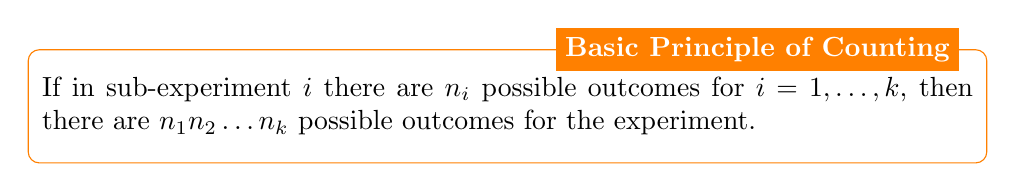
\begin{tikzpicture}
\node [rounded-box] (box){\begin{minipage}{0.975\textwidth}
    If in sub-experiment $i$ there are $n_i$ possible outcomes for $i = 1, \dots, k$, then there are $n_1 n_2 \dots n_k$ possible outcomes for the experiment.
\end{minipage}};
\node[rounded-box-title, left=10pt] at (box.north east) {Basic Principle of Counting};
\end{tikzpicture}

\begin{paracol}{2}

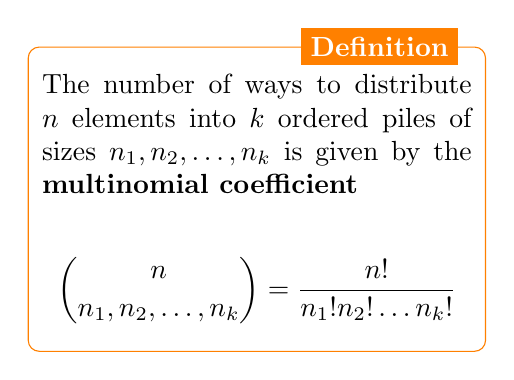
\begin{tikzpicture}
\node [rounded-box] (box){\begin{minipage}{0.45\textwidth}
    The number of ways to distribute $n$ elements into $k$ ordered piles of sizes $n_1, n_2, \dots, n_k$ is given by the \textbf{multinomial coefficient}

    $$\binom{n}{n_1, n_2, \dots, n_k} = \frac{n!}{n_1! n_2! \dots n_k!}$$
\end{minipage}};
\node[rounded-box-title, left=10pt] at (box.north east) {Definition};
\end{tikzpicture}

\switchcolumn

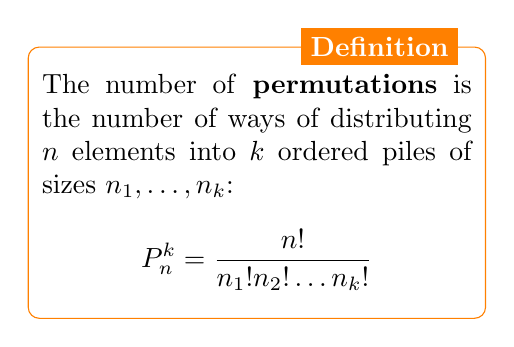
\begin{tikzpicture}
\node [rounded-box] (box){\begin{minipage}{0.45\textwidth}
    The number of \textbf{permutations} is the number of ways of distributing $n$ elements into $k$ ordered piles of sizes $n_1, \dots, n_k$:

    $$P_n^k = \frac{n!}{n_1! n_2! \dots n_k!}$$
\end{minipage}};
\node[rounded-box-title, left=10pt] at (box.north east) {Definition};
\end{tikzpicture}

\switchcolumn

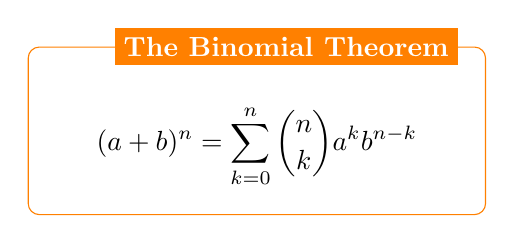
\begin{tikzpicture}
\node [rounded-box] (box){\begin{minipage}{0.45\textwidth}
    $$(a + b)^n = \sum_{k=0}^n \binom{n}{k} a^k b^{n-k}$$
\end{minipage}};
\node[rounded-box-title, left=10pt] at (box.north east) {The Binomial Theorem};
\end{tikzpicture}

\switchcolumn

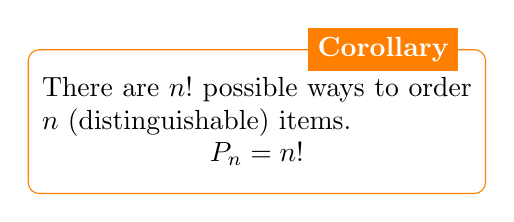
\begin{tikzpicture}
\node [rounded-box] (box){\begin{minipage}{0.45\textwidth}
    There are $n!$ possible ways to order $n$ (distinguishable) items.

    \vspace{-12.5pt}

    $$P_n = n!$$
\end{minipage}};
\node[rounded-box-title, left=10pt] at (box.north east) {Corollary};
\end{tikzpicture}

\switchcolumn

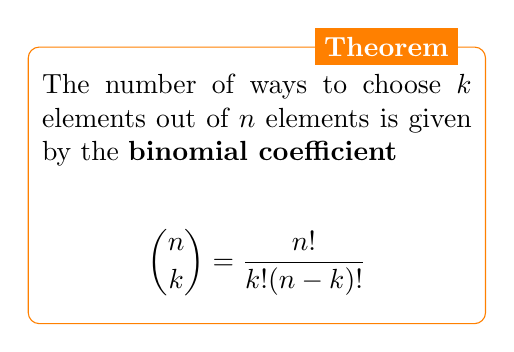
\begin{tikzpicture}
\node [rounded-box] (box){\begin{minipage}{0.45\textwidth}
    The number of ways to choose $k$ elements out of $n$ elements is given by the \textbf{binomial coefficient} \\

    $$\binom{n}{k} = \frac{n!}{k! (n-k)!}$$
\end{minipage}};
\node[rounded-box-title, left=10pt] at (box.north east) {Theorem};
\end{tikzpicture}

\switchcolumn

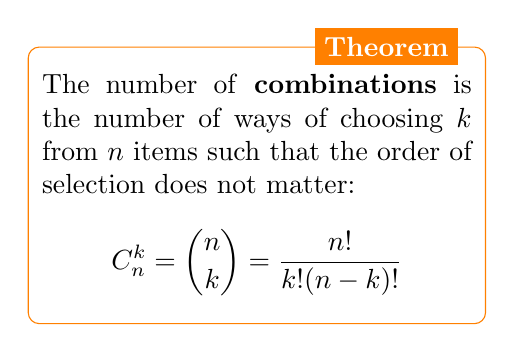
\begin{tikzpicture}
\node [rounded-box] (box){\begin{minipage}{0.45\textwidth}
    The number of \textbf{combinations} is the number of ways of choosing $k$ from $n$ items such that the order of selection does not matter:

    $$C_n^k = \binom{n}{k} = \frac{n!}{k! (n-k)!}$$
\end{minipage}};
\node[rounded-box-title, left=10pt] at (box.north east) {Theorem};
\end{tikzpicture}

\end{paracol}

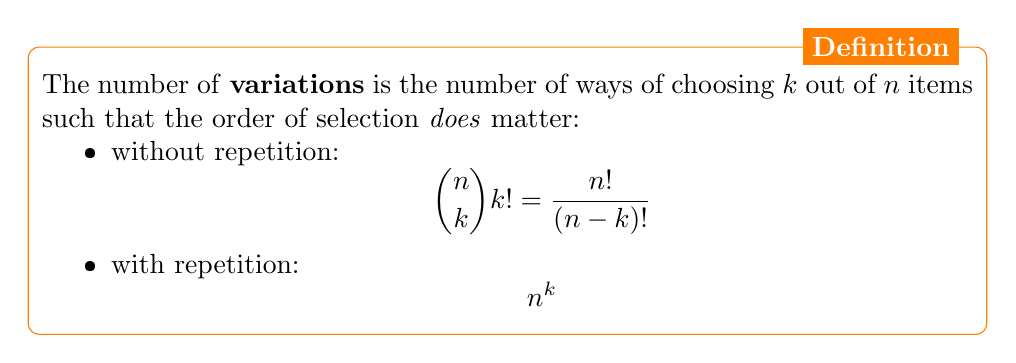
\begin{tikzpicture}
\node [rounded-box] (box){\begin{minipage}{0.975\textwidth}
    The number of \textbf{variations} is the number of ways of choosing $k$ out of $n$ items such that the order of selection \textit{does} matter:

    \begin{itemize}
        \item without repetition:
        $$\binom{n}{k} k! = \frac{n!}{(n-k)!}$$
        \item with repetition:
        $$n^k$$
    \end{itemize}
\end{minipage}};
\node[rounded-box-title, left=10pt] at (box.north east) {Definition};
\end{tikzpicture}

\section{Axioms of Probability}

\subsection{Probability Spaces}

\begin{paracol}{2}

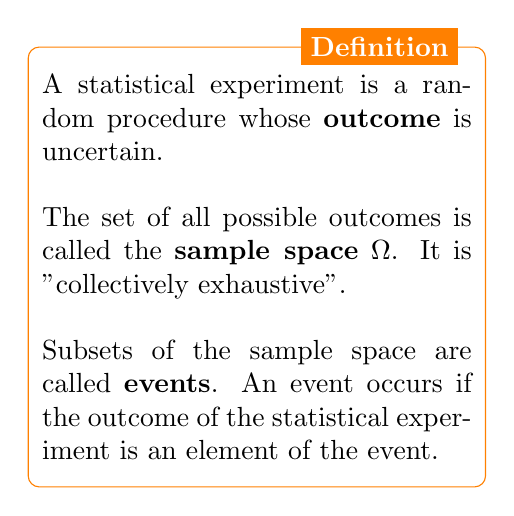
\begin{tikzpicture}
\node [rounded-box] (box){\begin{minipage}{0.45\textwidth}
    A statistical experiment is a random procedure whose \textbf{outcome} is uncertain. \\

    The set of all possible outcomes is called the \textbf{sample space} $\Omega$. It is "collectively exhaustive". \\

    Subsets of the sample space are called \textbf{events}. An event occurs if the outcome of the statistical experiment is an element of the event.
\end{minipage}};
\node[rounded-box-title, left=10pt] at (box.north east) {Definition};
\end{tikzpicture}

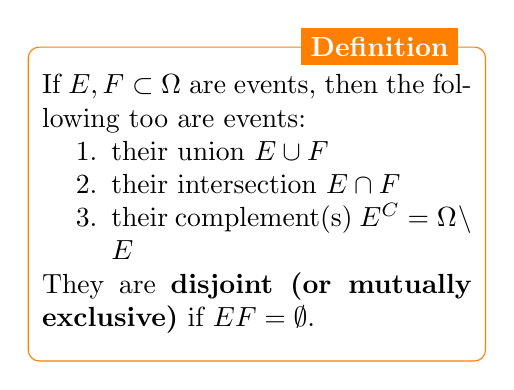
\begin{tikzpicture}
\node [rounded-box] (box){\begin{minipage}{0.45\textwidth}
    If $E, F \subset \Omega$ are events, then the following too are events:

    \begin{enumerate}
        \item their union $E \cup F$
        \item their intersection $E \cap F$
        \item their complement(s) $E^C = \Omega \setminus E$
    \end{enumerate}

    They are \textbf{disjoint (or mutually exclusive)} if $EF = \emptyset$.
\end{minipage}};
\node[rounded-box-title, left=10pt] at (box.north east) {Definition};
\end{tikzpicture}

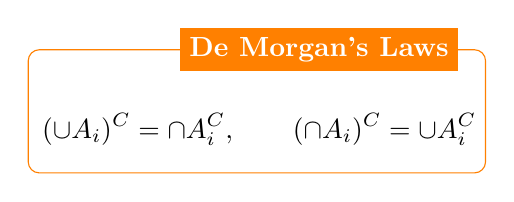
\begin{tikzpicture}
\node [rounded-box] (box){\begin{minipage}{0.45\textwidth}
    $$( \cup A_i )^C = \cap A_i^C , \qquad ( \cap A_i )^C = \cup A_i^C$$
\end{minipage}};
\node[rounded-box-title, left=10pt] at (box.north east) {De Morgan's Laws};
\end{tikzpicture}

\switchcolumn

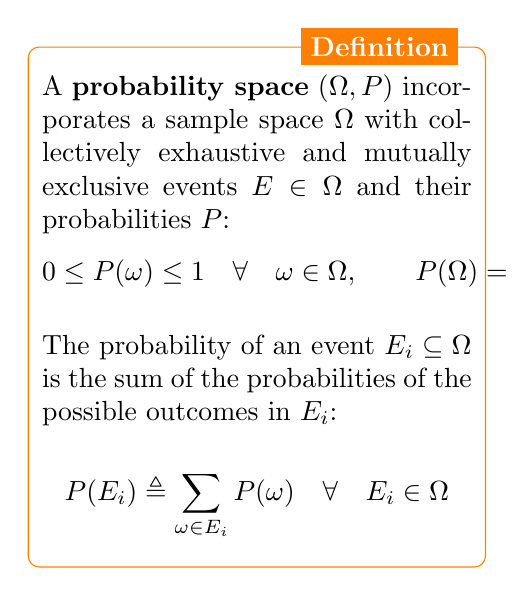
\begin{tikzpicture}
\node [rounded-box] (box){\begin{minipage}{0.45\textwidth}
    A \textbf{probability space} $(\Omega, P)$ incorporates a sample space $\Omega$ with collectively exhaustive and mutually exclusive events $E \in \Omega$ and their probabilities $P$:

    \vspace{-15pt}

    $$0 \leq P(\omega) \leq 1 \quad \forall \quad \omega \in \Omega, \qquad P(\Omega) = \sum_{\omega \in \Omega} P(\omega) = 1$$

    \vspace{-5pt}

    The probability of an event $E_i \subseteq \Omega$ is the sum of the probabilities of the possible outcomes in $E_i$:

    \vspace{-5pt}

    $$P(E_i) \triangleq \sum_{\omega \in E_i} P(\omega) \quad \forall \quad E_i \in \Omega$$
\end{minipage}};
\node[rounded-box-title, left=10pt] at (box.north east) {Definition};
\end{tikzpicture}

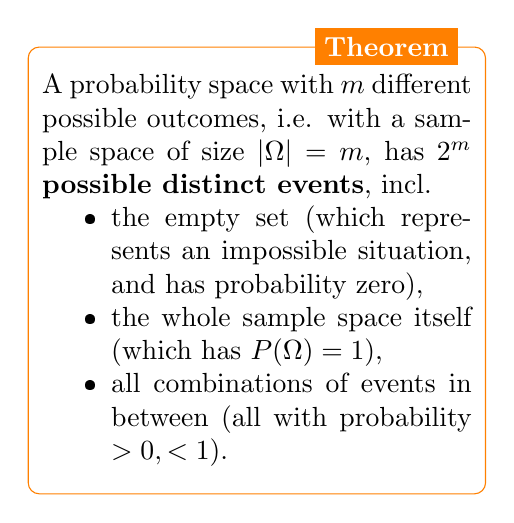
\begin{tikzpicture}
\node [rounded-box] (box){\begin{minipage}{0.45\textwidth}
    A probability space with $m$ different possible outcomes, i.e. with a sample space of size $| \Omega | = m$, has
    $2^m$
    \textbf{possible distinct events}, incl.

    \begin{itemize}
        \item the empty set (which represents an impossible situation, and has probability zero),
        \item the whole sample space itself (which has $P(\Omega) = 1$),
        \item all combinations of events in between (all with probability $> 0, < 1$).
    \end{itemize}
\end{minipage}};
\node[rounded-box-title, left=10pt] at (box.north east) {Theorem};
\end{tikzpicture}

\end{paracol}

\newpage

\subsection{Probability Functions}

\begin{paracol}{2}

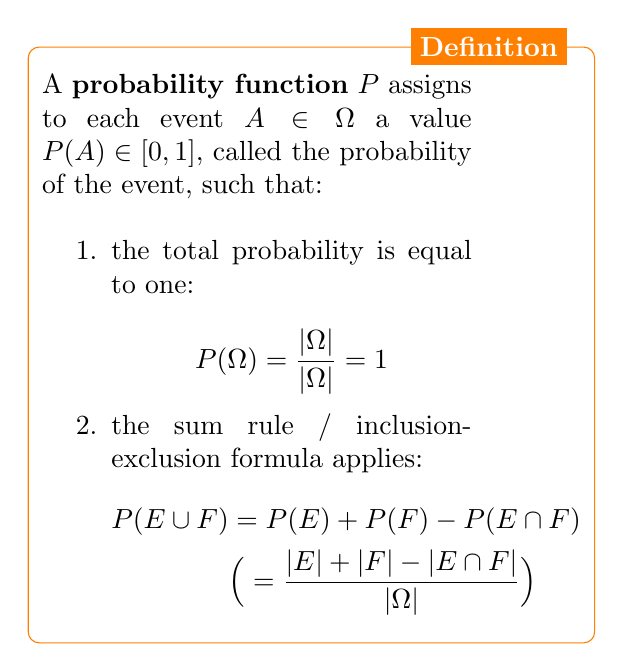
\begin{tikzpicture}
\node [rounded-box] (box){\begin{minipage}{0.45\textwidth}
    A \textbf{probability function} $P$ assigns to each event $A \in \Omega$ a value $P(A) \in [0, 1]$, called the probability of the event, such that: \\

    \begin{enumerate}
        \item the total probability is equal to one:

        $$P(\Omega) = \frac{| \Omega |}{| \Omega |} = 1$$
        
        \item the sum rule / inclusion-exclusion formula applies: \begin{align*}
            P(E \cup F) & = P(E) + P(F) - P(E \cap F) \\
            & \Big( = \frac{| E | + | F | - | E \cap F |}{| \Omega |} \Big)
        \end{align*}
    \end{enumerate}
\end{minipage}};
\node[rounded-box-title, left=10pt] at (box.north east) {Definition};
\end{tikzpicture}

\switchcolumn

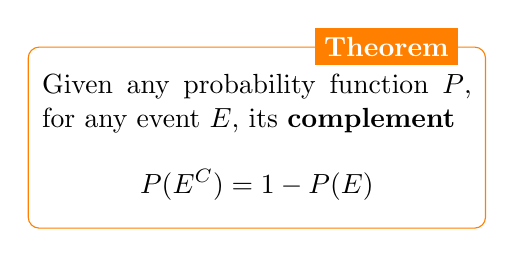
\begin{tikzpicture}
\node [rounded-box] (box){\begin{minipage}{0.45\textwidth}
    Given any probability function $P$, for any event $E$, its \textbf{complement}

    $$P(E^C) = 1 - P(E)$$
\end{minipage}};
\node[rounded-box-title, left=10pt] at (box.north east) {Theorem};
\end{tikzpicture}

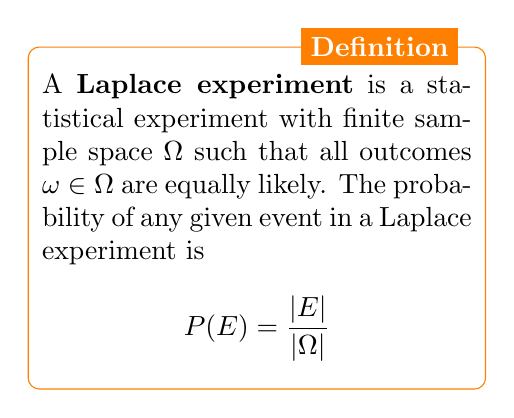
\begin{tikzpicture}
\node [rounded-box] (box){\begin{minipage}{0.45\textwidth}
    A \textbf{Laplace experiment} is a statistical experiment with finite sample space $\Omega$ such that all outcomes $\omega \in \Omega$ are equally likely. The probability of any given event in a Laplace experiment is

    $$P(E) = \frac{| E |}{| \Omega |}$$
\end{minipage}};
\node[rounded-box-title, left=10pt] at (box.north east) {Definition};
\end{tikzpicture}

\end{paracol}

\subsection{Conditional Probability}

\begin{paracol}{2}

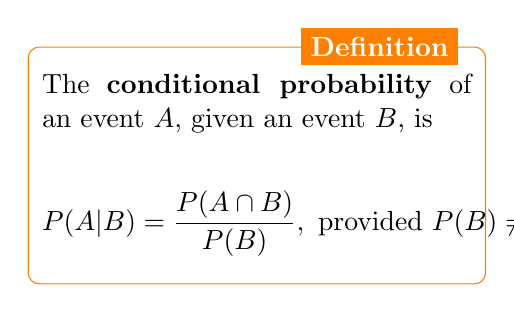
\begin{tikzpicture}
\node [rounded-box] (box){\begin{minipage}{0.45\textwidth}
    The \textbf{conditional probability} of an event $A$, given an event $B$, is

    $$P(A | B) = \frac{P(A \cap B)}{P(B)}, \text{ provided } P(B) \neq 0$$
\end{minipage}};
\node[rounded-box-title, left=10pt] at (box.north east) {Definition};
\end{tikzpicture}

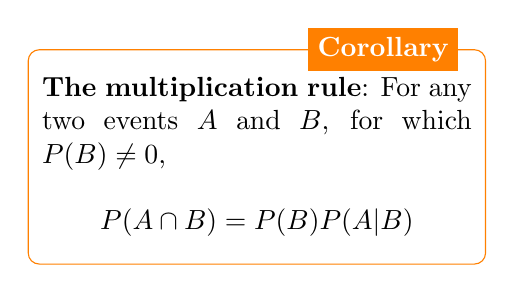
\begin{tikzpicture}
\node [rounded-box] (box){\begin{minipage}{0.45\textwidth}
    \textbf{The multiplication rule}: For any two events $A$ and $B$, for which $P(B) \neq 0$,

    $$P(A \cap B) = P(B) P(A | B)$$
\end{minipage}};
\node[rounded-box-title, left=10pt] at (box.north east) {Corollary};
\end{tikzpicture}

\switchcolumn

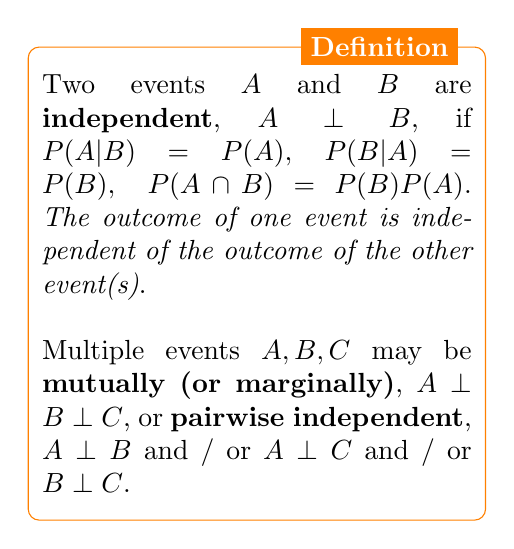
\begin{tikzpicture}
\node [rounded-box] (box){\begin{minipage}{0.45\textwidth}
    Two events $A$ and $B$ are \textbf{independent}, $A \perp B$, if $P(A | B) = P(A), \quad P(B | A) = P(B), \quad P(A \cap B) = P(B) P(A)$. \textit{The outcome of one event is independent of the outcome of the other event(s)}. \\

    Multiple events $A, B, C$ may be \textbf{mutually (or marginally)}, $A \perp B \perp C$, or \textbf{pairwise independent}, $A \perp B$ and / or $A \perp C$ and / or $B \perp C$.
\end{minipage}};
\node[rounded-box-title, left=10pt] at (box.north east) {Definition};
\end{tikzpicture}

\textbf{Example}:  With a fair coin, let's say that we just tossed it five times and tails turned up all five times. Is it more likely now that we'll see heads? No, because the previous outcome doesn't tell us anything about the outcome of a new toss.

\end{paracol}

\begin{paracol}{2}

\textbf{Example}: Random variables $W, I$ are not independent:

\begin{verbatim}
>>> prob_W_I = np.array([[1/2, 0], [0, 1/6], [0, 1/3]])
>>> prob_W_I
array([[0.5       , 0.        ],
       [0.        , 0.16666667],
       [0.        , 0.33333333]])
>>> prob_W = prob_W_I.sum(axis=1)
>>> prob_I = prob_W_I.sum(axis=0)
>>> prob_W
array([0.5       , 0.16666667, 0.33333333])
>>> prob_I
array([0.5, 0.5])
>>> np.outer(prob_W, prob_I)
array([[0.25      , 0.25      ],
       [0.08333333, 0.08333333],
       [0.16666667, 0.16666667]])
\end{verbatim}

\switchcolumn

\textbf{Example}: Random variables $X, Y$ are independent:

\begin{verbatim}
>>> prob_X_Y = np.array([[1/4, 1/4], [1/12, 1/12], [1/6, 1/6]])
>>> prob_X_Y
array([[0.25      , 0.25      ],
       [0.08333333, 0.08333333],
       [0.16666667, 0.16666667]])
>>> prob_X = prob_X_Y.sum(axis=1)
>>> prob_Y = prob_X_Y.sum(axis=0)
>>> prob_X
array([0.5       , 0.16666667, 0.33333333])
>>> prob_Y
array([0.5, 0.5])
>>> np.outer(prob_X, prob_Y)
array([[0.25      , 0.25      ],
       [0.08333333, 0.08333333],
       [0.16666667, 0.16666667]])
\end{verbatim}

\end{paracol}

\subsection{Law of Total Probability and Bayes' Theorem}

\begin{paracol}{2}

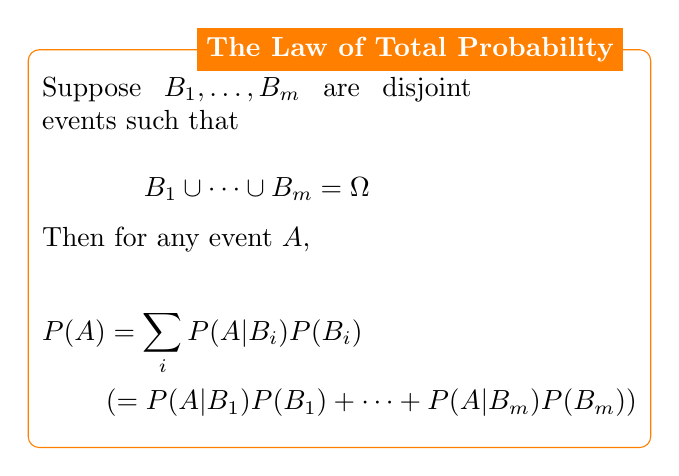
\begin{tikzpicture}
\node [rounded-box] (box){\begin{minipage}{0.45\textwidth}
    Suppose $B_1, \dots, B_m$ are disjoint events such that

    $$B_1 \cup \dots \cup B_m = \Omega$$

    Then for any event $A$,

    \begin{align*}
        P(A) & = \sum_i P(A | B_i) P(B_i) \\
        & ( = P(A | B_1) P(B_1) + \dots + P(A | B_m) P(B_m) )
    \end{align*}
\end{minipage}};
\node[rounded-box-title, left=10pt] at (box.north east) {The Law of Total Probability};
\end{tikzpicture}

\switchcolumn

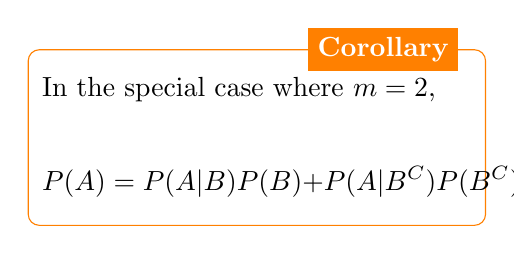
\begin{tikzpicture}
\node [rounded-box] (box){\begin{minipage}{0.45\textwidth}
    In the special case where $m = 2$,

    $$P(A) = P(A | B) P(B) + P(A | B^C) P(B^C)$$
\end{minipage}};
\node[rounded-box-title, left=10pt] at (box.north east) {Corollary};
\end{tikzpicture}

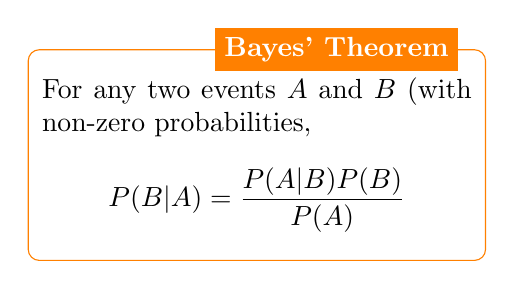
\begin{tikzpicture}
\node [rounded-box] (box){\begin{minipage}{0.45\textwidth}
    For any two events $A$ and $B$ (with non-zero probabilities,

    $$P(B | A) = \frac{P(A | B) P(B)}{P(A)}$$
\end{minipage}};
\node[rounded-box-title, left=10pt] at (box.north east) {Bayes' Theorem};
\end{tikzpicture}

\end{paracol}
 \newpage
\section{Discrete Random Variables}

\begin{paracol}{2}

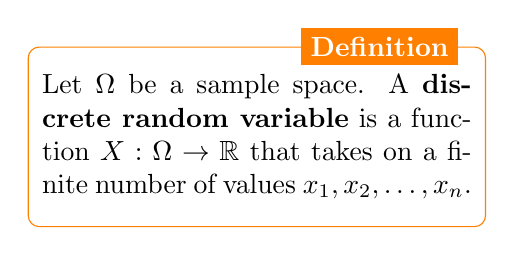
\begin{tikzpicture}
\node [rounded-box] (box){\begin{minipage}{0.45\textwidth}
    Let $\Omega$ be a sample space. A \textbf{discrete random variable} is a function $X : \Omega \rightarrow \mathbb{R}$ that takes on a finite number of values $x_1, x_2, \dots, x_n$.
\end{minipage}};
\node[rounded-box-title, left=10pt] at (box.north east) {Definition};
\end{tikzpicture}

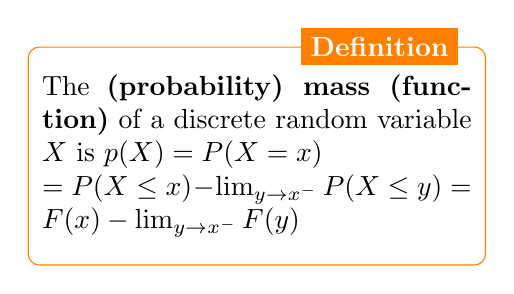
\begin{tikzpicture}
\node [rounded-box] (box){\begin{minipage}{0.45\textwidth}
    The \textbf{(probability) mass (function)} of a discrete random variable $X$ is $p(X) = P(X = x)$

    $= P(X \leq x) - \lim_{y \rightarrow x^-} P(X \leq y) = F(x) - \lim_{y \rightarrow x^-} F(y)$
\end{minipage}};
\node[rounded-box-title, left=10pt] at (box.north east) {Definition};
\end{tikzpicture}

\switchcolumn

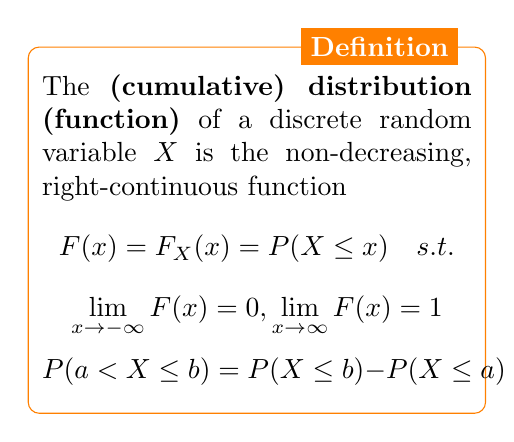
\begin{tikzpicture}
\node [rounded-box] (box){\begin{minipage}{0.45\textwidth}
    The \textbf{(cumulative) distribution (function)} of a discrete random variable $X$ is the non-decreasing, right-continuous function
    $$F(x) = F_X(x) = P(X \leq x) \quad s.t.$$
    $$\lim_{x \rightarrow -\infty} F(x) = 0, \lim_{x \rightarrow \infty} F(x) = 1$$
    $$P(a < X \leq b) = P(X \leq b) - P(X \leq a) = F(b) - F(a)$$
\end{minipage}};
\node[rounded-box-title, left=10pt] at (box.north east) {Definition};
\end{tikzpicture}

\end{paracol}

\subsection{Expectation and Variance}

The expectation is comparable to the centre of mass of an object - the point where it would balance.

The variance and standard deviation measure the spread of a probability distribution around the expectation. Specifically, the standard deviation is the distance from the mean, with 68\%, 95\% and 99.7\% of data points within one, two and three standard deviations from the expectation, respectively.

\begin{paracol}{2}

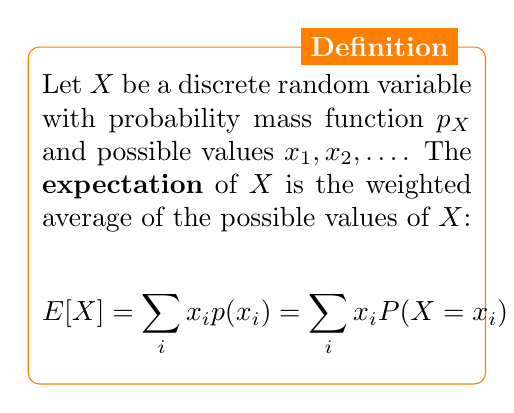
\begin{tikzpicture}
\node [rounded-box] (box){\begin{minipage}{0.45\textwidth}
    Let $X$ be a discrete random variable with probability mass function $p_X$ and possible values $x_1, x_2, \dots$. The \textbf{expectation} of $X$ is the weighted average of the possible values of $X$:

    $$E[X] = \sum_i{x_i p(x_i)} = \sum_i{x_i P(X=x_i)}$$
\end{minipage}};
\node[rounded-box-title, left=10pt] at (box.north east) {Definition};
\end{tikzpicture}

\switchcolumn

For the standard deviation, consider the expression $X - E[X]$. It is also a random variable, so one could take its expectation, however, by definition it will always occur that $E[X - E[X]] = 0$. Therefore, a more practical definition is:

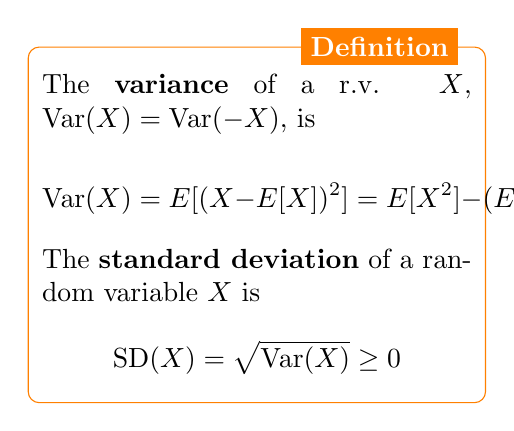
\begin{tikzpicture}
\node [rounded-box] (box){\begin{minipage}{0.45\textwidth}
    The \textbf{variance} of a r.v. $X$, $\text{Var}(X) = \text{Var}(-X)$, is

    \vspace{-5pt}

    $$\text{Var}(X) = E[(X - E[X])^2] = E[X^2] - (E[X])^2 \geq 0$$

    The \textbf{standard deviation} of a random variable $X$ is

    $$\text{SD}(X) = \sqrt{\text{Var}(X)} \geq 0$$
\end{minipage}};
\node[rounded-box-title, left=10pt] at (box.north east) {Definition};
\end{tikzpicture}

\switchcolumn

\textbf{Example}: Consider the random variable $X$ for which $P(X = -1) = P(X = 1) = p, P(X = 0) = 1-2p, 0 < p < \frac{1}{2}$.

\vspace{-20pt}

\begin{align*}
    E[X] & = (-1) \cdot p + 1 \cdot p + 0 \cdot (1-2p) = 0 \\
    \text{Var}(X) & = (-1)^2 \cdot p + 1^2 \cdot p + 0^2 \cdot (1-2p) - (E[X])^2 = 2p
\end{align*}

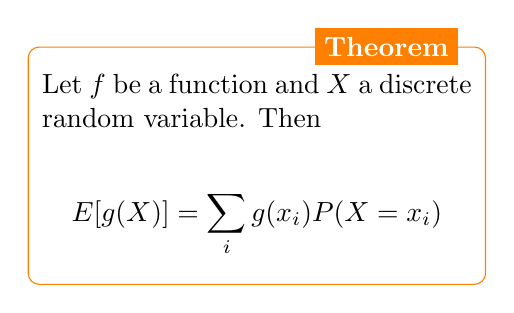
\begin{tikzpicture}
\node [rounded-box] (box){\begin{minipage}{0.45\textwidth}
    Let $f$ be a function and $X$ a discrete random variable. Then

    $$E[g(X)] = \sum_i{g(x_i) P(X = x_i)}$$
\end{minipage}};
\node[rounded-box-title, left=10pt] at (box.north east) {Theorem};
\end{tikzpicture}

Note: In general, $E[g(X)] \neq g(E[X])$.


\begin{tikzpicture}
\node [rounded-box] (box){\begin{minipage}{0.45\textwidth}
    If $E[g(X)]$ and $g(E[X])$ are finite, and $g(x)$ is a \textbf{convex} function on $R_X$, i.e. $f''(x) \geq 0$, then
    
    $$E[g(X)] \geq g(E[X])$$

    If $E[g(X)]$ and $g(E[X])$ are finite, and $g(x)$ is a \textbf{concave} function on $R_X$, i.e. $f''(x) \leq 0$, then
    
    $$E[g(X)] \leq g(E[X])$$
\end{minipage}};
\node[rounded-box-title, left=10pt] at (box.north east) {Jensen's Inequaltiy};
\end{tikzpicture}

\textbf{Example}:

Let $g(x) = x^a \quad \forall \quad a \in \mathbb{R}$. Then $f''(x) = a(a-1)x^{a-2} > 0 \iff a < 0 \text{ or } a > 1$. Therefore,

$$
\begin{cases}
    E[X^a] \geq (E[X])^a & \text{ if } a < 0 \text{ or } a > 1 \\
    E[X^a] = (E[X])^a & \text{ if } a = 0 \text{ or } a = 1 \\
    E[X^a] \leq (E[X])^a & \text{ if } 0 < a < 1
\end{cases}
$$

\switchcolumn

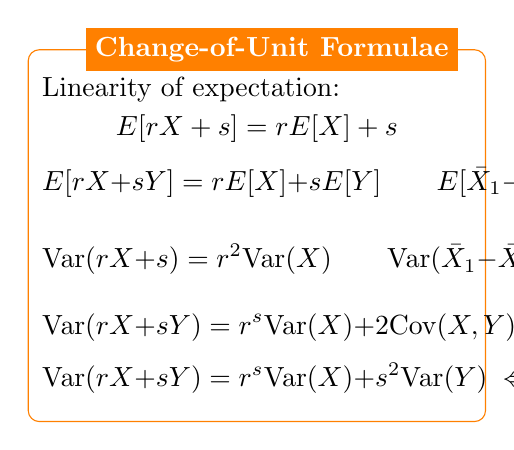
\begin{tikzpicture}
\node [rounded-box] (box){\begin{minipage}{0.45\textwidth}
    Linearity of expectation:

    \vspace{-10pt}

    $$E[rX + s] = r E[X] + s$$

    \vspace{-20pt}
    
    $$E[rX + sY] = r E[X] + s E[Y] \qquad E[\bar{X}_1 - \bar{X}_2] = \mu_1 - \mu_2$$

    \vspace{-20pt}

    $$\text{Var}(rX + s) = r^2 \text{Var}(X) \qquad \text{Var}(\bar{X}_1 - \bar{X}_2) = \frac{\sigma_1^2}{n_1} + \frac{\sigma_2^2}{n_2}$$

    \vspace{-20pt}

    $$\text{Var}(rX + sY) = r^s \text{Var}(X) + 2 \text{Cov}(X, Y) + s^2 \text{Var}(Y)$$

    \vspace{-25pt}

    $$\text{Var}(rX + sY) = r^s \text{Var}(X) + s^2 \text{Var}(Y) \iff X \perp Y$$
\end{minipage}};
\node[rounded-box-title, left=10pt] at (box.north east) {Change-of-Unit Formulae};
\end{tikzpicture}

\textbf{Proofs}:

    \vspace{-10pt}

\begin{align*}
    E[rX + s] & = \sum_i{(r x_i + s) P(X = x_i)} \\
    & = \sum_i{r x_i P(X = x_i)} + \sum_i{s P(X = x_i)} \\
    & = r \sum_i{x_i P(X = x_i)} + s \sum_i{P(X = x_i)} \\
    & = r E[X] + s \\
\end{align*}

\vspace{-30pt}

\begin{align*}
    \text{Var}(rX + s) & = E[(rX + s)^2] - (E[rX + s])^2 \\
    & = E[r^2 X^2 + 2rsX + s^2] - (rE[X] + s)^2 \\
    & = (r^2 E[X^2] + 2rsE[X] + s^2) \\
    & \quad \quad - (r^2 (E[X])^2 + 2rsE[X] + s^2) \\
    & = r^2 (E[X^2] - (E[X])^2) \\
    & = r^2 \text{Var}(X)
\end{align*}

\end{paracol}

\newpage

\subsection{Discrete Distributions}

\begin{paracol}{2}

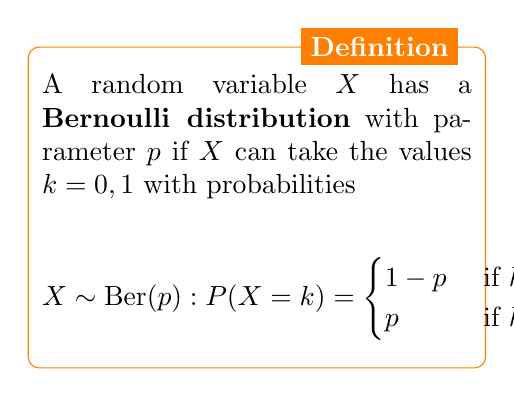
\begin{tikzpicture}
\node [rounded-box] (box){\begin{minipage}{0.45\textwidth}
    A random variable $X$ has a \textbf{Bernoulli distribution} with parameter $p$ if $X$ can take the values $k = 0, 1$ with probabilities

    $$X \sim \text{Ber}(p) :
    P(X = k) = \begin{cases}
        1 - p & \text{ if } k = 0 \\
        p & \text{ if } k = 1
    \end{cases}
    $$
\end{minipage}};
\node[rounded-box-title, left=10pt] at (box.north east) {Definition};
\end{tikzpicture}

The geometric distribution describes how many \textit{independent} Bernoulli experiments are needed until the first success.

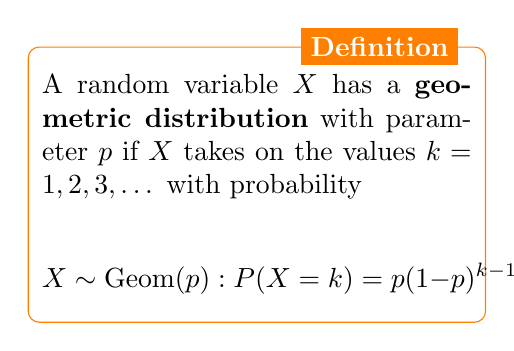
\begin{tikzpicture}
\node [rounded-box] (box){\begin{minipage}{0.45\textwidth}
    A random variable $X$ has a \textbf{geometric distribution} with parameter $p$ if $X$ takes on the values $k = 1, 2, 3, \dots$ with probability

    $$X \sim \text{Geom}(p):
    P(X = k) = p (1-p)^{k-1}
    $$
\end{minipage}};
\node[rounded-box-title, left=10pt] at (box.north east) {Definition};
\end{tikzpicture}

\textbf{Example}: The geometric distribution is memory-less:

\vspace{-20pt}

\begin{align*}
    P(X = 11 | X > 7) & = \frac{P(X = 11 \cap X > 7)}{P(X > 7)} \\
    & = \frac{P(X = 11)}{P(X > 7)} \\
    & = \frac{p (1-p)^{11-1}}{(1-p)^7} \\
    & = p (1-p)^3
\end{align*}

The binomial distribution models the number of successes in a sequence of length $n$.

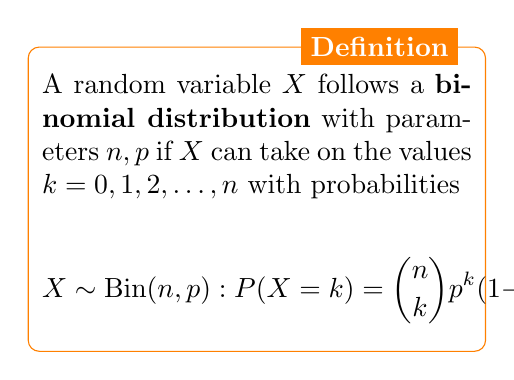
\begin{tikzpicture}
\node [rounded-box] (box){\begin{minipage}{0.45\textwidth}
    A random variable $X$ follows a \textbf{binomial distribution} with parameters $n, p$ if $X$ can take on the values $k = 0, 1, 2, \dots, n$ with probabilities

    $$X \sim \text{Bin}(n, p) :
    P(X = k) = \binom{n}{k} p^k (1-p)^{n-k}
    $$
\end{minipage}};
\node[rounded-box-title, left=10pt] at (box.north east) {Definition};
\end{tikzpicture}

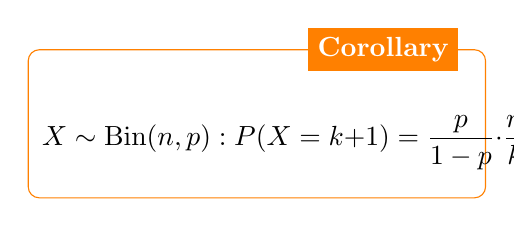
\begin{tikzpicture}
\node [rounded-box] (box){\begin{minipage}{0.45\textwidth}
    $$X \sim \text{Bin}(n, p) : P(X = k + 1) = \frac{p}{1-p} \cdot \frac{n-k}{k+1} \cdot P(X = k)$$
\end{minipage}};
\node[rounded-box-title, left=10pt] at (box.north east) {Corollary};
\end{tikzpicture}

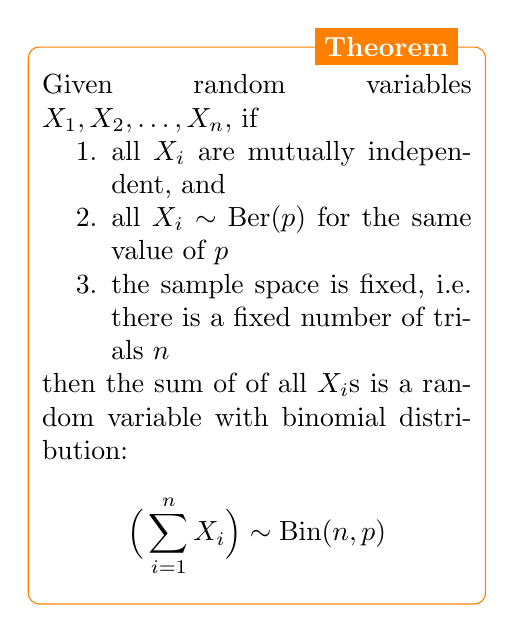
\begin{tikzpicture}
\node [rounded-box] (box){\begin{minipage}{0.45\textwidth}
    Given random variables $X_1, X_2, \dots, X_n$, if

    \begin{enumerate}
        \item all $X_i$ are mutually independent, and
        \item all $X_i \sim \text{Ber}(p)$ for the same value of $p$
        \item the sample space is fixed, i.e. there is a fixed number of trials $n$
    \end{enumerate}

    then the sum of of all $X_i$s is a random variable with binomial distribution:

    $$
    \Big( \sum_{i=1}^n{X_i} \Big) \sim \text{Bin}(n, p)
    $$
\end{minipage}};
\node[rounded-box-title, left=10pt] at (box.north east) {Theorem};
\end{tikzpicture}

The \textbf{negative binomial distribution} models the number of independent $\text{Ber}(p)$ trials until the $r^{th}$ success: $\sum_{i=1}^r \text{Geom}(p)$.

The \textbf{hypergeometric distribution} models the number of red balls drawn when we draw $n$ balls out of $m$ red balls and $N-m$ blue balls.

\switchcolumn

The Poisson distribution models the number of random occurrences of a specific event over a fixed interval (time, space).

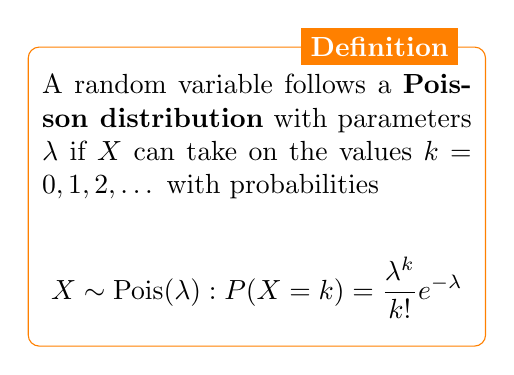
\begin{tikzpicture}
\node [rounded-box] (box){\begin{minipage}{0.45\textwidth}
    A random variable follows a \textbf{Poisson distribution} with parameters $\lambda$ if $X$ can take on the values $k = 0, 1, 2, \dots$ with probabilities

    $$X \sim \text{Pois}(\lambda) :
    P(X = k) = \frac{\lambda^k}{k!} e^{-\lambda}
    $$
\end{minipage}};
\node[rounded-box-title, left=10pt] at (box.north east) {Definition};
\end{tikzpicture}

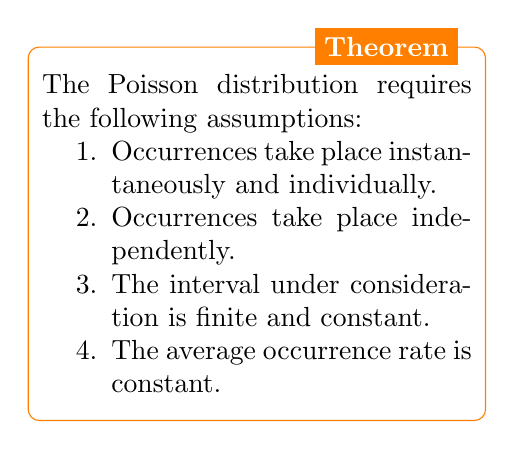
\begin{tikzpicture}
\node [rounded-box] (box){\begin{minipage}{0.45\textwidth}
    The Poisson distribution requires the following assumptions:

    \begin{enumerate}
        \item Occurrences take place instantaneously and individually.
        \item Occurrences take place independently.
        \item The interval under consideration is finite and constant.
        \item The average occurrence rate is constant.
    \end{enumerate}
\end{minipage}};
\node[rounded-box-title, left=10pt] at (box.north east) {Theorem};
\end{tikzpicture}

\textbf{Derivation}:

Divide a given interval into $n$ sub-intervals. The occurrence of an event in each sub-interval is either $0$ or $1$:

$$X_m \sim \text{Ber}\Big(\frac{\lambda}{n}\Big), m = 1, \dots, n$$

By independence, the total number of occurrences in the discrete interval is

$$Y_n = X_1 + \dots + X_n \sim \text{Bin}\Big(n, \frac{\lambda}{n}\Big)$$

That is, $Y_n \sim \text{Bin}(n, \frac{\lambda}{n})$ has probability mass function

$$P(Y_n = k) = \binom{n}{k} \Big(\frac{\lambda}{n}\Big)^k \Big(1 - \frac{\lambda}{n}\Big)^{n-k}$$

The Poisson distribution is the $\lim_{n \rightarrow \infty} \text{Bin}(n, p), \lambda = np$ (and, \textbf{for large} $n$ \textbf{and small} $p$, \textbf{can be used as an approximation for the binomial distribution} $\text{Bin}(n, p)$):

\vspace{-25pt}

\begin{align*}
    \lim_{n \rightarrow \infty}{P(Y_n = k)} & = \lim_{n \rightarrow \infty}{\binom{n}{k} \Big(\frac{\lambda}{n}\Big)^k \Big(1 - \frac{\lambda}{n}\Big)^{n-k}} \\
    & = \frac{\lambda^k}{k!} e^{-\lambda}
\end{align*}

\vspace{20pt}

\begin{center}
\begin{tabular}{c|c|c|c}
    Distribution & PMF & $E[X]$ & $\text{Var}(X)$ \\
    \hline
    $\text{Ber}(p)$ & $\begin{cases} p & x = 1 \\ 1-p & p = 0 \end{cases}$ & $p$ & $p(1-p)$ \\[0.5cm]
    $\text{Geom}(p)$ & $p (1-p)^{(k-1)}$ & $1/p$ & $(1-p)/p^2$ \\[0.5cm]
    \text{Bin}(n, p) & $\binom{n}{k} p^k (1-p)^{(n-k)}$ & $np$ & $np(1-p)$ \\[0.5cm]
    $\text{Pois}(\lambda)$ & $\lambda^k e^{-\lambda} / k!$ & $\lambda$ & $\lambda$ \\[0.5cm]
    $\text{NBin}(r, p)$ & $\binom{n-1}{r-1} (1-p)^{n-r} p^r$ & $r/p$ & $r(1-p)/p^2$ \\[0.5cm]
    $\text{HG}(N, m, n)$ & $\binom{m}{k} \binom{N-m}{n-k} / \binom{N}{n}$ & $nm/M$ &
\end{tabular}
\end{center}

\end{paracol}
 \newpage
\section{Continuous Random Variables}

\begin{paracol}{2}

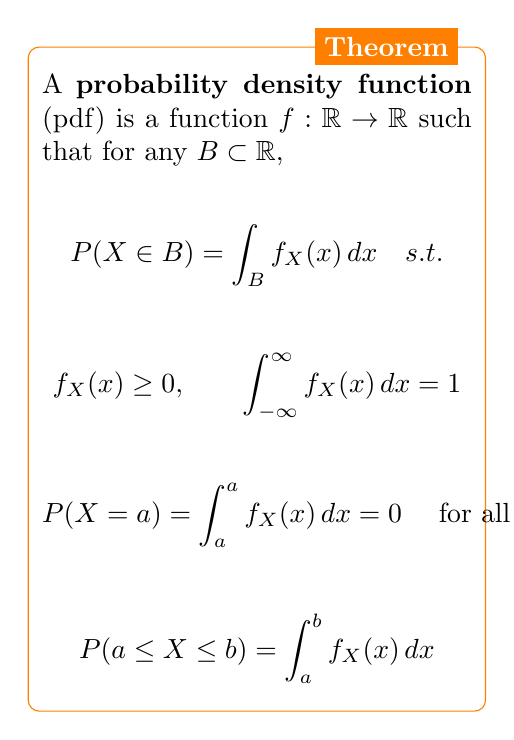
\begin{tikzpicture}
\node [rounded-box] (box){\begin{minipage}{0.45\textwidth}
    A \textbf{probability density function} (pdf) is a function $f : \mathbb{R} \rightarrow \mathbb{R}$ such that for any $B \subset \mathbb{R}$,

    $$P(X \in B) = \int_B f_X(x) \, dx \quad s.t.$$

    $$f_X(x) \geq 0, \qquad \int_{-\infty}^{\infty} f_X(x) \,dx = 1$$

    $$P(X = a) = \int_a^a f_X(x) \,dx = 0 \quad \text{ for all } a \in \mathbb{R}$$

    $$P(a \leq X \leq b) = \int_a^b f_X(x) \,dx$$
\end{minipage}};
\node[rounded-box-title, left=10pt] at (box.north east) {Theorem};
\end{tikzpicture}

\switchcolumn

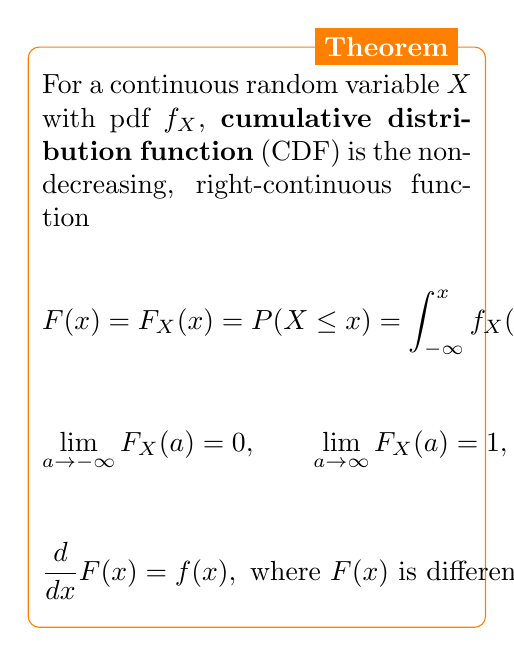
\begin{tikzpicture}
\node [rounded-box] (box){\begin{minipage}{0.45\textwidth}
    For a continuous random variable $X$ with pdf $f_X$, \textbf{cumulative distribution function} (CDF) is the non-decreasing, right-continuous function

    $$F(x) = F_X(x) = P(X \leq x) = \int_{-\infty}^x f_X(x) \,dx \quad s.t.$$

    $$\lim_{a \rightarrow -\infty} F_X(a) = 0, \qquad \lim_{a \rightarrow \infty} F_X(a) = 1, \qquad F(\infty) = 1$$
    
    $$\frac{d}{dx}F(x) = f(x), \text{ where } F(x) \text{ is differentiable}$$
\end{minipage}};
\node[rounded-box-title, left=10pt] at (box.north east) {Theorem};
\end{tikzpicture}

\end{paracol}

The PDF represents the instantaneous probability density at a point, while the CDF represents the accumulated probability up to that point. This relationship is a direct consequence of the Fundamental Theorem of Calculus.

\subsection{Expectation and Variance}

\begin{paracol}{2}

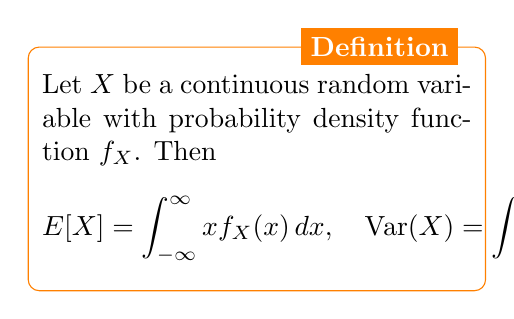
\begin{tikzpicture}
\node [rounded-box] (box){\begin{minipage}{0.45\textwidth}
    Let $X$ be a continuous random variable with probability density function $f_X$. Then

    \vspace{-10pt}

    $$E[X] = \int_{-\infty}^{\infty} x f_X(x) \,dx,
    \quad
    \text{Var}(X) = \int (x - E[X])^2 f_X(x) \,dx$$
\end{minipage}};
\node[rounded-box-title, left=10pt] at (box.north east) {Definition};
\end{tikzpicture}

\switchcolumn

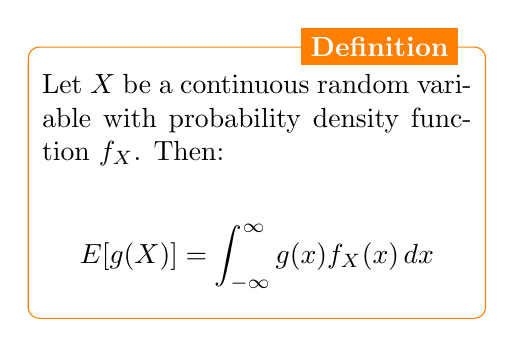
\begin{tikzpicture}
\node [rounded-box] (box){\begin{minipage}{0.45\textwidth}
    Let $X$ be a continuous random variable with probability density function $f_X$. Then:

    $$E[g(X)] = \int_{-\infty}^{\infty} g(x) f_X(x) \,dx$$
\end{minipage}};
\node[rounded-box-title, left=10pt] at (box.north east) {Definition};
\end{tikzpicture}

\end{paracol}

Jensen's inequality and the change-of-unit formula apply just like in the discrete case.

\subsection{The Exponential Distribution}

\begin{paracol}{2}

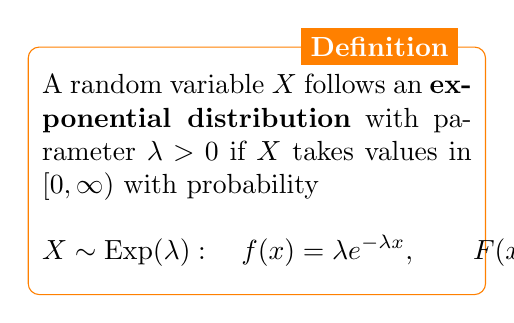
\begin{tikzpicture}
\node [rounded-box] (box){\begin{minipage}{0.45\textwidth}
    A random variable $X$ follows an \textbf{exponential distribution} with parameter $\lambda > 0$ if $X$ takes values in $[0, \infty)$ with probability

    \vspace{-10pt}

    $$X \sim \text{Exp}(\lambda) : \quad
    f(x) = \lambda e^{-\lambda x}, \qquad F(x) = 1 - e^{-\lambda x}$$
\end{minipage}};
\node[rounded-box-title, left=10pt] at (box.north east) {Definition};
\end{tikzpicture}

The exponential distribution models the waiting time between events that are modelled by a Poisson distribution.

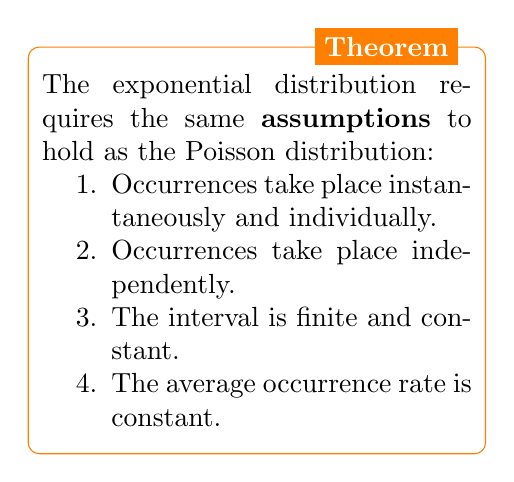
\begin{tikzpicture}
\node [rounded-box] (box){\begin{minipage}{0.45\textwidth}
    The exponential distribution requires the same \textbf{assumptions} to hold as the Poisson distribution:

    \begin{enumerate}
        \item Occurrences take place instantaneously and individually.
        \item Occurrences take place independently.
        \item The interval is finite and constant.
        \item The average occurrence rate is constant.
    \end{enumerate}
\end{minipage}};
\node[rounded-box-title, left=10pt] at (box.north east) {Theorem};
\end{tikzpicture}

The exponential distribution also shares the geometric distribution's property of memorylessness:

\begin{itemize}
    \item $\text{Geom}(p)$ counts discrete "failures" until "successes".
    \item $\text{Exp}(\lambda)$ measures continuous time between "events".
\end{itemize}

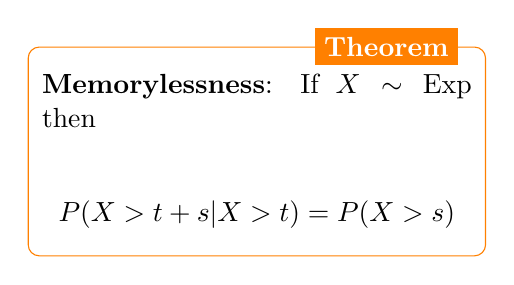
\begin{tikzpicture}
\node [rounded-box] (box){\begin{minipage}{0.45\textwidth}
    \textbf{Memorylessness}: If $X \sim \text{Exp}$ then

    $$P(X > t + s | X > t) = P(X > s)$$
\end{minipage}};
\node[rounded-box-title, left=10pt] at (box.north east) {Theorem};
\end{tikzpicture}

\switchcolumn

\textbf{Derivation}:

Assume we expect six customers per hour, or one customer every 10 minutes:

$$N \sim \text{Poisson}(6), N_\frac{1}{6} \sim \text{Poisson}(1)$$

In general, the "number of events in $t$ time units" $N_t$ is thus:

$$N_t \sim \text{Poisson}(\lambda t)$$

The probability of waiting at least $t$ units between events is the probability of zero events occurring in $t$ units, as modelled by the Poisson distribution:

$$P(X > t) = P(N_t = 0) = e^{-\lambda t}$$

Therefore, the cumulative distribution function of the exponential distribution, the cumulative waiting time, is

$$F(t) = P(X \leq t) = 1 - P(X > t) = 1 - e^{-\lambda t}$$

Differentiation gives the probability density function.

The expectation can be found by found by integration by parts:

$$E[X] = \int_0^\infty x \lambda e^{-\lambda x} \,dx = \frac{1}{\lambda}$$

\end{paracol}

The \textbf{Gamma distribution} is the sum of exponentials: $\Gamma(n, \lambda) = \sum_{i=1}^n \text{Exp}(\lambda)$

\subsection{The Pareto Distribution}

\begin{paracol}{2}

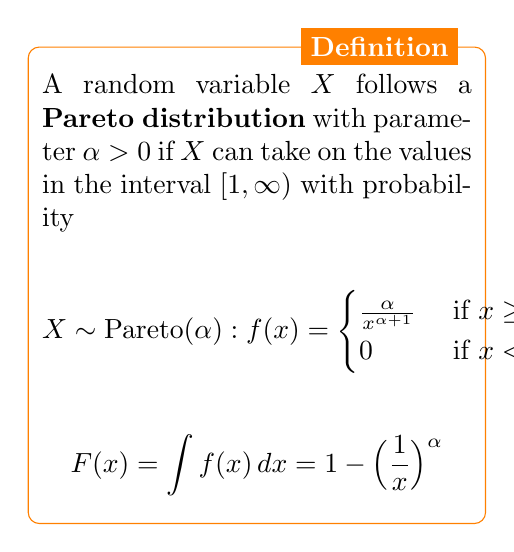
\begin{tikzpicture}
\node [rounded-box] (box){\begin{minipage}{0.45\textwidth}
    A random variable $X$ follows a \textbf{Pareto distribution} with parameter $\alpha > 0$ if $X$ can take on the values in the interval $[1, \infty)$ with probability

    $$X \sim \text{Pareto}(\alpha) :
    f(x) = \begin{cases}
        \frac{\alpha}{x^{\alpha+1}} & \text{ if } x \geq 1 \\
        0 & \text{ if } x < 1
    \end{cases}$$

    $$F(x) = \int f(x) \,dx = 1 - \Big( \frac{1}{x} \Big)^\alpha$$
\end{minipage}};
\node[rounded-box-title, left=10pt] at (box.north east) {Definition};
\end{tikzpicture}

TODO: The $0.10^\text{th}$ quantile is such that $F(x) = 0.10$ (for all distributions).

\switchcolumn

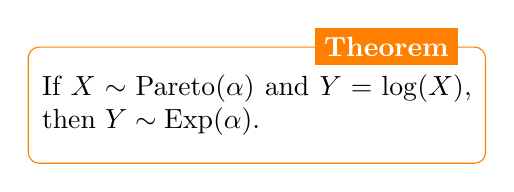
\begin{tikzpicture}
\node [rounded-box] (box){\begin{minipage}{0.45\textwidth}
    If $X \sim \text{Pareto}(\alpha)$ and $Y = \log(X)$, then $Y \sim \text{Exp}(\alpha)$.
\end{minipage}};
\node[rounded-box-title, left=10pt] at (box.north east) {Theorem};
\end{tikzpicture}

\textbf{Proof}:

\vspace{-30pt}

\begin{align*}
    F_Y(y) & = P(Y \leq y) \\
    & = P(\log(X) \leq y) \\
    & = P(X \leq e^y) \\
    & = F_X(e^y) \\
    & = 1 - (\frac{1}{e^y})^\alpha \\
    & = 1 - e^{-\alpha y}
\end{align*}

\end{paracol}

\subsection{The Normal Distribution}

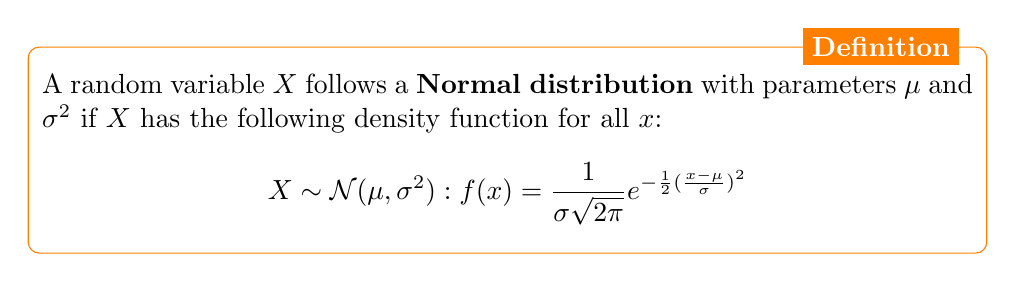
\begin{tikzpicture}
\node [rounded-box] (box){\begin{minipage}{0.975\textwidth}
    A random variable $X$ follows a \textbf{Normal distribution} with parameters $\mu$ and $\sigma^2$ if $X$ has the following density function for all $x$:

    $$X \sim \mathcal{N}(\mu, \sigma^2) :
    f(x) = \frac{1}{\sigma \sqrt{2 \pi}} e^{-\frac{1}{2}(\frac{x-\mu}{\sigma})^2}$$
\end{minipage}};
\node[rounded-box-title, left=10pt] at (box.north east) {Definition};
\end{tikzpicture}

The integral of this Gaussian function cannot be written using
elementary functions. However, the standard normal distribution can be used to calculate probabilities!

\begin{paracol}{2}

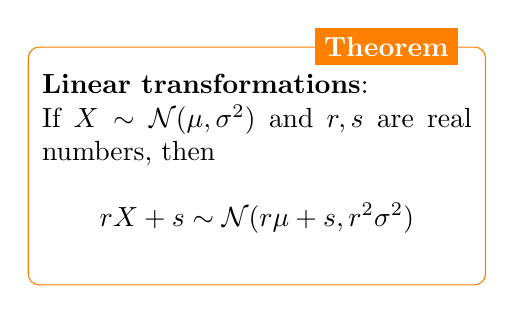
\begin{tikzpicture}
\node [rounded-box] (box){\begin{minipage}{0.45\textwidth}
    \textbf{Linear transformations}:
    
    If $X \sim \mathcal{N}(\mu, \sigma^2)$ and $r, s$ are real numbers, then

    $$rX + s \sim \mathcal{N}(r\mu + s, r^2 \sigma^2)$$

    \vspace{2.5pt}
\end{minipage}};
\node[rounded-box-title, left=10pt] at (box.north east) {Theorem};
\end{tikzpicture}

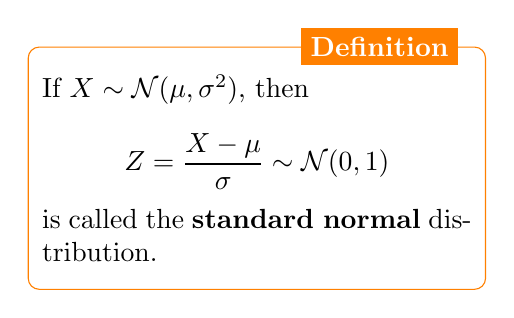
\begin{tikzpicture}
\node [rounded-box] (box){\begin{minipage}{0.45\textwidth}
    If $X \sim \mathcal{N}(\mu, \sigma^2)$, then

    $$Z = \frac{X - \mu}{\sigma} \sim \mathcal{N}(0, 1)$$

    is called the \textbf{standard normal} distribution.
\end{minipage}};
\node[rounded-box-title, left=10pt] at (box.north east) {Definition};
\end{tikzpicture}

\switchcolumn

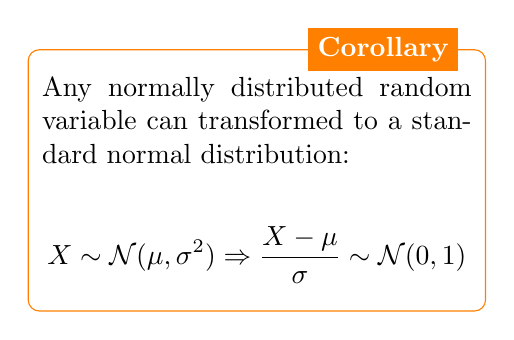
\begin{tikzpicture}
\node [rounded-box] (box){\begin{minipage}{0.45\textwidth}
    Any normally distributed random variable can transformed to a standard normal distribution:

    $$X \sim \mathcal{N}(\mu, \sigma^2) \Rightarrow \frac{X - \mu}{\sigma} \sim \mathcal{N}(0, 1)$$
\end{minipage}};
\node[rounded-box-title, left=10pt] at (box.north east) {Corollary};
\end{tikzpicture}

\begin{tikzpicture}
\node [rounded-box] (box){\begin{minipage}{0.45\textwidth}
    $$\Phi(-x) = 1 - \Phi(x) \iff P(X \leq -x) = P(X > x)$$
    $$F(x) = P(X \leq x) = P\Big( \frac{X - \mu}{\sigma} \leq \frac{x - \mu}{\sigma} \Big) = \Phi\Big( \frac{x - \mu}{\sigma} \Big)$$
\end{minipage}};
\node[rounded-box-title, left=10pt] at (box.north east) {Theorem};
\end{tikzpicture}

\end{paracol}

\vspace{5pt}

\begin{center}
\begin{tabular}{c|c|c|c}
    Distribution & PDF & $E[X]$ & $\text{Var}(X)$ \\

    \hline

    $\text{Uni}(a, b)$ & $\frac{1}{b-a}, \quad a < x < b$ & $\frac{1}{2}(a + b)$ & $\frac{1}{12}(b - a)^2$ \\[0.5cm]

    $\text{Exp}(\lambda)$ & $\lambda e^{-\lambda x}, \quad x > 0$ & $1 / \lambda$ & $1 / \lambda^2$ \\[0.5cm]

    $\text{Gamma}(n, \lambda)$ & $\frac{(\lambda x)^{n-1}}{\lambda e^{\lambda x}(n-1)!}, \quad x > 0$ & $n / \lambda$ & $n / \lambda^2$ \\[0.5cm]

    $\text{Pareto}(\alpha)$ & $\begin{cases}
        \frac{\alpha}{x^{\alpha+1}} & \text{ if } x \geq 1 \\
        0 & \text{ if } x < 1
    \end{cases}$ & $\begin{cases}
        \infty & \text{ for } \alpha \leq 1 \\
        \frac{\alpha}{\alpha - 1} & \text{ for } \alpha > 1
    \end{cases}$ & $\begin{cases}
        \infty & \text{ for } \alpha \leq 2 \\
        \frac{\alpha}{(\alpha - 1)^2 (\alpha - 2)} & \text{ for } \alpha > 2
    \end{cases}$ \\[0.5cm]

    $\mathcal{N}(\mu, \sigma^2)$ & $\frac{1}{\sqrt{2 \pi \sigma^2}} e^{- \frac{(x - \mu)^2}{2 \sigma^2}}$ & $\mu$ & $\sigma^2$ \\[0.5cm]

    Standard normal & $\frac{1}{\sqrt{2 \pi}} e^{- \frac{x^2}{2}}$ & $0$ & $1$
\end{tabular}
\end{center}

\vspace{5pt}

\begin{paracol}{2}

\begin{tikzpicture}
\node [rounded-box] (box){\begin{minipage}{0.45\textwidth}
    $S_n \sim \text{Bin}(n, p)$ converges to a standard normal

    $$
    \lim_{n \rightarrow \infty} P \Big( a \leq \frac{S_n - np}{\sqrt{np (1-p)}} \leq b \Big) = \Phi(b) - \Phi(a)
    $$
\end{minipage}};
\node[rounded-box-title, left=10pt] at (box.north east) {DeMoivre-Laplace Theorem};
\end{tikzpicture}

\switchcolumn

Thus, there are two \textbf{approximations to the binomial distribution}:

\begin{itemize}
    \item The Poisson distribution is a good approximation when $n$ is large and $p$ is small.

    \item The standard normal distribution is a good approximation when $np (1-p)$ is large.
\end{itemize}

\end{paracol}
 \newpage
\section{Multivariate Random Variables}

\subsection{Joint Distributions}

\begin{paracol}{2}

\begin{tikzpicture}
\node [rounded-box] (box){\begin{minipage}{0.45\textwidth}
    Let $X$ and $Y$ be two discrete random variables. The \textbf{joint probability mass function} $p$ of $X$ and $Y$ is the function $p : \mathbb{R}^2 \rightarrow [0, 1]$ defined by

    $$p_{X, Y}(x, y) = P(X = x, Y = y) \text{ for all } x, y$$

    Their \textbf{joint cumulative distribution function} is the function $F_{X, Y} : \mathbb{R}^2 \rightarrow [0, 1]$ defined by

    $$F_{X, Y}(x, y) = P(X \leq x, Y \leq y) \text{ for all } x, y$$
\end{minipage}};
\node[rounded-box-title, left=10pt] at (box.north east) {Definition};
\end{tikzpicture}

\begin{tikzpicture}
\node [rounded-box] (box){\begin{minipage}{0.45\textwidth}
    Let $p_{X, Y}(x, y)$ be the joint probability mass function of $(X, Y)$. Then the \textbf{marginal probability mass functions} of $X$ and $Y$ are given by

    $$p_X(x) = P(X = x) = \sum_y{p_{X, Y}(x, y)}$$
    
    $$p_Y(y) = P(Y = y) = \sum_x{p_{X, Y}(x, y)}$$

    This generalises to multiple random variables, e.g. $p_{X, Y}(x, y) = \sum_z p_{X, Y, Z}(x, y, z)$, etc.
\end{minipage}};
\node[rounded-box-title, left=10pt] at (box.north east) {Definition};
\end{tikzpicture}

NB: The inverse is not true: In general, \textit{the joint distribution cannot be computed based on the knowledge of marginal distributions}. Intuitively, we would be missing key information about the dependencies between $X$ and $Y$.

\textbf{Example}: Consider random variables $(S, T)$ and $(U, V)$, where $S$ and $U$ have the same distribution, and $T$ and $V$ have the same distribution. However, $(S, T)$ and $(U, V)$ do not necessarily have the same joint distribution:

\begin{center}
\begin{tabular}{c|c|c}
S / T & 1 & 0 \\
\hline
sunny & 1 / 2 & 0 \\
\hline
rainy & 0 & 1 / 6 \\
\hline
snowy & 0 & 1 / 3
\end{tabular}
\quad
\begin{tabular}{c|c|c}
U / V & 1 & 0 \\
\hline
sunny & 1 / 4 & 1 / 4 \\
\hline
rainy & 1 / 12 & 1 / 12 \\
\hline
snowy & 1 / 6 & 1 / 6
\end{tabular}
\end{center}

\begin{tikzpicture}
\node [rounded-box] (box){\begin{minipage}{0.45\textwidth}
    Let $X$ and $Y$ be two discrete random variables with joint probability mass function $p_{X, Y}(x, y)$. The \textbf{expectation} of the joint random vector $(X, Y)$ is the vector

    $$E[(X, Y)] = \sum_{x, y}{(x, y) p_{X, Y}(x, y)}$$
\end{minipage}};
\node[rounded-box-title, left=10pt] at (box.north east) {Definition};
\end{tikzpicture}

\begin{tikzpicture}
\node [rounded-box] (box){\begin{minipage}{0.45\textwidth}
    Let $g$ be a function of two variables. Then

    $$E[g(X, Y)] = \sum_{x, y}{g(x, y) p_{X, Y}(x, y)}$$
\end{minipage}};
\node[rounded-box-title, left=10pt] at (box.north east) {Theorem};
\end{tikzpicture}

\switchcolumn

\begin{tikzpicture}
\node [rounded-box] (box){\begin{minipage}{0.45\textwidth}
    Let $X$ and $Y$ be two continuous random variables. The \textbf{joint probability density function} $f_{X, Y}(x, y)$ must satisfy the probability axioms:

    \begin{enumerate}
        \item It is a non-negative function.
        \item The volume below its graph is 1.
    \end{enumerate}

    \vspace{5pt}

    Thus, the \textbf{joint cumulative distribution function} is

    \vspace{-7.5pt}

    $$F_{X, Y}(x, y) = P(X \leq x, Y \leq y) = \int_{-\infty}^x \int_{-\infty}^y f_{X, Y}(x, y) \,dy\,dx$$
\end{minipage}};
\node[rounded-box-title, left=10pt] at (box.north east) {Definition};
\end{tikzpicture}

\begin{tikzpicture}
\node [rounded-box] (box){\begin{minipage}{0.45\textwidth}
    Let $f_{X, Y}(x, y)$ be the joint probability density function of $(X, Y)$. Then the \textbf{marginal probability density functions} of $X$ and $Y$ are given by

    $$f_X(x) = P(X = x) = \int_{-\infty}^\infty f_{X, Y}(x, y) \,dy$$
    
    $$f_Y(y) = P(Y = y) = \int_{-\infty}^\infty f_{X, Y}(x, y) \,dx$$

    The \textbf{marginal cumulative distribution functions} of $X$ and $Y$ are thus derived as follows:

    \vspace{-20pt}

    \begin{align*}
        P(X \leq x) & = P(X \leq x, Y < \infty)
        = \int_{-\infty}^x \int_{-\infty}^\infty f_{X, Y}(x, y) \,dy\,dx \\
        & = \int_{-\infty}^x f_X(x) \,dx
        = F_X(x)
    \end{align*}
\end{minipage}};
\node[rounded-box-title, left=10pt] at (box.north east) {Definition};
\end{tikzpicture}

\begin{tikzpicture}
\node [rounded-box] (box){\begin{minipage}{0.45\textwidth}
For two continuous jointly-distributed $X, Y$,

\vspace{-15pt}

$$P(a \leq X \leq b, c \leq Y \leq d) = \int_a^b \int_c^d f_{X, Y}(x, y) \,dy\,dx$$
\end{minipage}};
\node[rounded-box-title, left=10pt] at (box.north east) {Definition};
\end{tikzpicture}

\begin{tikzpicture}
\node [rounded-box] (box){\begin{minipage}{0.45\textwidth}
    If $X$ and $Y$ are two continuous random variables with joint probability density function $f_{X, Y}$, then

    $$E[g(X, Y)] = \int_{-\infty}^\infty \int_{-\infty}^\infty g(x, y) f_{X, Y}(x, y) \,dx\,dy$$
\end{minipage}};
\node[rounded-box-title, left=10pt] at (box.north east) {Theorem};
\end{tikzpicture}

\begin{tikzpicture}
\node [rounded-box] (box){\begin{minipage}{0.45\textwidth}
    The distribution of the \textbf{sum of two random variables} is

    \vspace{-10pt}

    $$F_{X + Y}(a) = \int_{-\infty}^\infty F_X(a - y) f_Y(y) \, dy$$

    and its density is

    $$f_{X + Y}(a) = \int_{-\infty}^\infty f_X(a - y) f_Y(y) \, dy$$
\end{minipage}};
\node[rounded-box-title, left=10pt] at (box.north east) {Theorem};
\end{tikzpicture}

\end{paracol}

In particular, the sums of random variables following the following discrete and continuous distributions are defined as:

\vspace{-20pt}

$$
\sum_{i=1}^n \text{Ber}(p) = \text{Bin}(n, p)
\qquad
\sum_{i=1}^n \text{Geom}(p) = \text{NegBin}(n, p)
\qquad
\sum_{i=1}^n \text{Poisson}(\lambda_i) = \text{Poisson}\Big(\sum_{i=1}^n \lambda_i \Big) = \text{Poisson}\Big(\lambda_1 + \dots + \lambda_n \Big)
$$

$$
\sum_{i=1}^n \text{Exp}(\lambda) = \Gamma(n, \lambda)
\qquad \qquad
\sum_{i=1}^n \mathcal{N}(\mu_i, \sigma_i^2) = \mathcal{N}\Big(\sum_{i=1}^n \mu_i, \sum_{i=1}^n \sigma_i^2\Big) = \mathcal{N}\Big(\mu_1 + \dots + \mu_n, \sigma_1^2 + \dots + \sigma_n^2\Big)
$$

\newpage

\subsection{Covariance and Correlation}

\begin{paracol}{2}

\begin{tikzpicture}
\node [rounded-box] (box){\begin{minipage}{0.45\textwidth}
    Let $X$ and $Y$ be two random variables. The \textbf{covariance} of $X$ and $Y$ is given by the expectation of the product of the deviations $X, Y$ from the mean

    \vspace{-10pt}

    \begin{align*}
        \text{Cov}(X, Y) & = E[(X - E[X]) (Y - E[Y])] \\
        & = E[XY - X E[Y] - Y E[X] + E[X] E[Y]] \\
        & = E[XY] - E[Y] E[X] - E[X] E[Y] + E[X] E[Y] \\
        & = E[XY] - E[X] E[Y] \\
        & (\text{where } E[XY] = \int_{-\infty}^\infty xy \, f_{X, Y}(x, y) \, dx \, dy )
    \end{align*}
\end{minipage}};
\node[rounded-box-title, left=10pt] at (box.north east) {Definition};
\end{tikzpicture}

\vspace{5pt}

\begin{tikzpicture}
\node [rounded-box] (box){\begin{minipage}{0.45\textwidth}
    The variance can thus be interpreted as the covariance of a random variable with itself:

    \vspace{-10pt}

    \begin{align*}
        \text{Cov}(X, X) & = E[X^2] - (E[X])^2 \\
        & = \text{Var}(X)
    \end{align*}
\end{minipage}};
\node[rounded-box-title, left=10pt] at (box.north east) {Corollary};
\end{tikzpicture}

\switchcolumn

\begin{tikzpicture}
\node [rounded-box] (box){\begin{minipage}{0.45\textwidth}
    The \textbf{change-of-unit formula} for the covariance is

    \vspace{-7.5pt}

    \begin{align*}
        \text{Cov}(rX + s, tY + u) & = E[rtXY + ruX + stY + su] \\
        & \quad - (r E[X] + s)(t E[Y] + u) \\
        & = rt E[XY] + ru E[X] + st E[Y] + su \\
        & \quad - (rt E[X] E[Y] + ru E[X] \\
        & \qquad + st E[Y] + su) \\
        & = rt \text{Cov}(X, Y)
    \end{align*}
\end{minipage}};
\node[rounded-box-title, left=10pt] at (box.north east) {Theorem};
\end{tikzpicture}

\begin{tikzpicture}
\node [rounded-box] (box){\begin{minipage}{0.45\textwidth}
    Let $X$ and $Y$ be two random variables. The \textbf{correlation}

    $$\rho(X, Y) = \frac{\text{Cov}(X, Y)}{\sqrt{\text{Var}(X) \text{Var}(Y)}}$$

    such that

    \begin{enumerate}
        \item $-1 \leq \rho(X, Y) \leq 1$ (i.e. it does not depend on units)
        \item $\rho(rX + s, tY + u) = \rho(X, Y)$ if $rt > 0$
    \end{enumerate}
\end{minipage}};
\node[rounded-box-title, left=10pt] at (box.north east) {Definition};
\end{tikzpicture}

\end{paracol}

\subsection{Independent Random Variables}

\begin{paracol}{2}

\begin{tikzpicture}
\node [rounded-box] (box){\begin{minipage}{0.45\textwidth}
    Let $X$ and $Y$ be two discrete random variables. $X$ and $Y$ are \textbf{independent} random variables if their joint probability mass function $p_{X, Y}$ is the product of the two marginal mass functions $p_X$ and $p_Y$:

    $$p_{X, Y}(x, y) = p_X(x) p_Y(y)$$
\end{minipage}};
\node[rounded-box-title, left=10pt] at (box.north east) {Definition};
\end{tikzpicture}

\begin{tikzpicture}
\node [rounded-box] (box){\begin{minipage}{0.45\textwidth}
    Let $X$ and $Y$ be two continuous random variables. $X$ and $Y$ are \textbf{independent} random variables if their joint probability density function $f_{X, Y}$ is the product of the two marginal density functions $f_X$ and $f_Y$:

    $$f_{X, Y}(x, y) = f_X(x) f_Y(y)$$
\end{minipage}};
\node[rounded-box-title, left=10pt] at (box.north east) {Definition};
\end{tikzpicture}

\switchcolumn

This has important implications for conditional probabilities:

\begin{tikzpicture}
\node [rounded-box] (box){\begin{minipage}{0.45\textwidth}
    If $X$ and $Y$ are independent random variables, \textbf{events} concerning $X$ and $Y$ are also independent.
\end{minipage}};
\node[rounded-box-title, left=10pt] at (box.north east) {Theorem};
\end{tikzpicture}

\begin{tikzpicture}
\node [rounded-box] (box){\begin{minipage}{0.45\textwidth}
    If $X$ and $Y$ are independent random variables, then they are \textbf{uncorrelated}:

    $$E[XY] = E[X] E[Y] \text{ and } \text{Cov}(X, Y) = 0 = \rho(X, Y)$$
\end{minipage}};
\node[rounded-box-title, left=10pt] at (box.north east) {Theorem};
\end{tikzpicture}

NB: The converse is not necessarily true; if two random variables are uncorrelated, they are not necessarily independent.

\end{paracol}

\subsection{The Bivariate Normal Distribution}

\begin{tikzpicture}
\node [rounded-box] (box){\begin{minipage}{0.975\textwidth}
    Let $X$ and $Y$ be two continuous random variables with joint probability density function

    $$f_{X, Y}(x, y) = \frac{1}{2 \pi \sigma_X \sigma_Y \sqrt{1 - \rho^2}} e^{-\frac{1}{2(1-\rho^2)}\big( (\frac{x-\mu_X}{\sigma_X})^2 + (\frac{y-\mu_Y}{\sigma_Y})^2 - 2 \rho (\frac{x-\mu_X}{\sigma_X}) (\frac{x-\mu_X}{\sigma_X}) \big)}$$

    where $\mu_X, \mu_Y \in \mathbb{R}, \sigma_X$ and $\sigma_Y$ are positive, and $-1 < \rho < 1$. Then $(X, Y)$ follow a \textbf{bivariate normal distribution}.
\end{minipage}};
\node[rounded-box-title, left=10pt] at (box.north east) {Definition};
\end{tikzpicture}

The \textbf{marginal distributions} are the standard normal ones. $\rho$ models the effect of two random variables on each other:

\vspace{-10pt}

$$\rho(X, Y) = \frac{E[XY] - E[X] E[Y]}{\sqrt{\text{Var}(X) \text{Var}(Y)}} = \frac{\int_{-\infty}^\infty \int_{-\infty}^\infty xy f_{X, Y}(x, y) \,dx\,dy - \mu_X \mu_Y}{\sigma_X \sigma_Y}$$

\vspace{-10pt}

\begin{tikzpicture}
\node [rounded-box] (box){\begin{minipage}{0.975\textwidth}
     While this is not generally true; for a bivariate normal distribution it can be shown that if $\rho = 0$, then $X$ and $Y$ are independent:

    $$
    f_{X, Y}(x, y) = \frac{1}{2 \pi \sigma_X \sigma_Y} e^{-\frac{1}{2}\big( (\frac{x-\mu_X}{\sigma_X})^2 + (\frac{y-\mu_Y}{\sigma_Y})^2 \big)} 
    = \frac{1}{\sqrt{2 \pi} \sigma_X} e^{- \frac{1}{2} (\frac{x-\mu_X}{\sigma_X})^2} \cdot \frac{1}{\sqrt{2 \pi} \sigma_Y} e^{- \frac{1}{2} (\frac{y-\mu_Y}{\sigma_Y})^2}
    = f_X(x) f_Y(y)
    $$
\end{minipage}};
\node[rounded-box-title, left=10pt] at (box.north east) {Theorem};
\end{tikzpicture}
 \newpage
\section{Conditional Distributions}

\subsection{Discrete Conditional Distributions}

\begin{paracol}{2}

\begin{tikzpicture}
\node [rounded-box] (box){\begin{minipage}{0.45\textwidth}
    Let $X$ and $Y$ be two discrete random variables. Then $X | Y = y$ is a \textbf{conditional random variable}. \\
    
    Its \textbf{discrete conditional pmf} is

    $$P(X = x | Y = y) = \frac{P(X = x \cap Y = y)}{P(Y = y)}$$

    or

    $$p_{X | Y}(x | y) = \frac{p_{X, Y}(x, y)}{p_Y(y)}$$

    for all $x$, provided $P(Y = y) \neq 0$.
\end{minipage}};
\node[rounded-box-title, left=10pt] at (box.north east) {Definition};
\end{tikzpicture}

\switchcolumn

\begin{tikzpicture}
\node [rounded-box] (box){\begin{minipage}{0.45\textwidth}
    Let $X$ and $Y$ be two discrete random variables such that

    $$P(X = x | Y = y) = \frac{P(X = x \cap Y = y)}{P(Y = y)}$$

    Then the marginal distribution can be calculated from just one conditional and one joint probability:

    $$P(Y = y) = \frac{P(X = x \cap Y = y)}{P(X = x | Y = y)}$$

    for any $x$.
\end{minipage}};
\node[rounded-box-title, left=10pt] at (box.north east) {Theorem};
\end{tikzpicture}

\end{paracol}

Furthermore, Bayes' Rule can be derived from this definition:

$$P(X = x \cap Y = y) = P(Y = y) P(X = x | Y = y) = P(X = x) P(Y = y | X = x)$$

$$P(Y = y | X = x) = P(X = x | Y = y) \frac{P(Y = y)}{P(X = x)}$$

\subsection{Continuous Conditional Distributions}

\begin{paracol}{2}

\begin{tikzpicture}
\node [rounded-box] (box){\begin{minipage}{0.45\textwidth}
    Let $X$ and $Y$ be two continuous random variables with joint density function $f_{X,Y}(x, y)$. Let $y$ be such that $f_Y(y) > 0$. Then the \textbf{conditional pdf} $f_{X | Y}$ is

    $$f_{X | Y}(x | y) = \frac{f_{X, Y}(x, y)}{f_Y(y)} = \frac{f_{X, Y}(x, y)}{\int f_{X, Y}(x, y) \,dx}$$

    and if $X, Y$ are independent:

    $$f_{X | Y}(x | y) = f_X(x)$$
\end{minipage}};
\node[rounded-box-title, left=10pt] at (box.north east) {Definition};
\end{tikzpicture}

\switchcolumn

Furthermore, as with any regular density function:

$$P(X \in A | Y = y) = \int_A f_{X | Y}(x | y) \,dx$$

$$F_{X | Y}(a | y) = P(X \leq a | Y = y) = \int_{-\infty}^a f_{X | Y}(x | y) \,dx$$

\end{paracol}

\subsection{Conditional Expectation and Variance}

\begin{paracol}{2}

\begin{tikzpicture}
\node [rounded-box] (box){\begin{minipage}{0.45\textwidth}
    Let $X$ and $Y$ be two continuous random variables and let $y$ be such that $f_Y(y) > 0$. Then

    $$E[X | (Y = y)] = \int x f_{X | Y}(x | y) \,dx$$

    $$\text{Var}[X | (Y = y)] = \int (x - E[X | (Y = y)])^2 f_{X | Y}(x | y) \,dx$$
\end{minipage}};
\node[rounded-box-title, left=10pt] at (box.north east) {Definition};
\end{tikzpicture}

\switchcolumn

\begin{tikzpicture}
\node [rounded-box] (box){\begin{minipage}{0.45\textwidth}
    Let $g(x, y)$ be a function.

    $$E[g(X, Y) | (Y = y)] = \int f(x, y) f_{X | Y}(x | y) \,dx$$
\end{minipage}};
\node[rounded-box-title, left=10pt] at (box.north east) {Theorem};
\end{tikzpicture}

\begin{tikzpicture}
\node [rounded-box] (box){\begin{minipage}{0.45\textwidth}
    $$X | (Y = y) \sim N \Big( \mu_X + \rho \frac{\sigma_X}{\sigma_Y}(y - \mu_Y), (1 - \rho^2) \sigma_X^2 \Big)$$
\end{minipage}};
\node[rounded-box-title, left=10pt] at (box.north east) {Theorem};
\end{tikzpicture}

\end{paracol}
 \newpage
\section{Limits}

\begin{paracol}{2}

\begin{tikzpicture}
\node [rounded-box] (box){\begin{minipage}{0.45\textwidth}
    For any random variable $X$ and positive constant $a > 0$,

    $$P( X \geq a) \leq \frac{E[X]}{a}$$
\end{minipage}};
\node[rounded-box-title, left=10pt] at (box.north east) {Markov Inequality};
\end{tikzpicture}

\textbf{Proof}: Since

$$E[X] = \int_0^\infty x \, f(x) \, dx \geq \int_a^\infty x \, f(x) \, dx,$$

it follows that

$$P( X \geq a) = \int_a^\infty f(x) \, dx \leq \frac{1}{a} \int_a^\infty x \, f(x) \, dx = \frac{E[X]}{a}$$

\switchcolumn

\begin{tikzpicture}
\node [rounded-box] (box){\begin{minipage}{0.45\textwidth}
    The probability that a random variable $X$ is more than a distance $a > 0$ from its expectation is

    $$P( | X - E[X] | \geq a) \leq \frac{\text{Var}(X)}{a^2}$$

    $$\text{If } a = k \sigma, \quad P(|X-\mu| \geq k \sigma) \leq \frac{1}{k^2}$$
\end{minipage}};
\node[rounded-box-title, left=10pt] at (box.north east) {Chebyshev's Inequality};
\end{tikzpicture}

\textbf{Proof}:

\vspace{-20pt}

\begin{align*}
    \text{Var}(X) & = E[(X-\mu)^2] = \int_{-\infty}^\infty (x-\mu)^2 f(x) \,dx \\
    & \geq \int_{|x-\mu| \geq a} (x-\mu)^2 f(x) \,dx \geq \int_{|x-\mu| \geq a} a^2 f(x) \,dx \\
    & = a^2 P(|X - \mu| \geq a)
\end{align*}

\switchcolumn

\subsection{The Law of Large Numbers (LLN)}

Convergence in probability is about the convergence of a given estimator $\bar{\theta}_n$ itself.

\begin{tikzpicture}
\node [rounded-box] (box){\begin{minipage}{0.45\textwidth}
    If $X_1, X_2, \dots, X_n$ are independent and all have the same distribution, then they constitute a \textbf{random sample}.
\end{minipage}};
\node[rounded-box-title, left=10pt] at (box.north east) {Definition};
\end{tikzpicture}

The larger the sample size, the lower the variance.

\begin{tikzpicture}
\node [rounded-box] (box){\begin{minipage}{0.45\textwidth}
    Consider a random sample $X_1, X_2, \dots, X_n$ with $E[X_i]=\mu, \text{Var}(X_i)=\sigma^2$.

    \vspace{-20pt}

    \begin{align*}
        E[\bar{X}_n] & = E[\frac{1}{n} (X_1 + X_2 + \dots + X_n)] \\
        & = \frac{1}{n} E[X_1 + X_2 + \dots + X_n] \\
        & = \frac{1}{n} n \mu \\
        & = \mu
    \end{align*}

    \vspace{-20pt}

    \begin{align*}
        \text{Var}(\bar{X}_n) & = \text{Var}\Big( \frac{1}{n} (X_1 + X_2 + \dots + X_n) \Big) \\
        & = \frac{1}{n^2} \text{Var}(X_1 + X_2 + \dots + X_n) \\
        & = \frac{1}{n^2} n \sigma^2 \qquad \text{(by independence)} \\
        & = \frac{\sigma^2}{n}
    \end{align*}
\end{minipage}};
\node[rounded-box-title, left=10pt] at (box.north east) {Theorem};
\end{tikzpicture}

By Chebyshev's inequality:

\vspace{-20pt}

$$P( | \bar{X}_n - E[\bar{X}_n] | \geq a) \leq \frac{\text{Var}(\bar{X}_n)}{a^2} = \frac{\text{Var}(X_i)}{a^2n}$$

\begin{tikzpicture}
\node [rounded-box] (box){\begin{minipage}{0.45\textwidth}
    If $X_1, X_2, \dots, X_n$ are independent, identically distributed random variables with $E[X_i] = \mu, \text{Var}(X_i) = \sigma^2$ for all $i$, then for any $a > 0$,

    $$\lim_{n \rightarrow \infty} P( | \bar{X}_n - \mu | \geq a) = 0$$
\end{minipage}};
\node[rounded-box-title, left=10pt] at (box.north east) {LLN};
\end{tikzpicture}

\textbf{Counter-example}: If the variance is infinite, e.g. as for some parameters of a Pareto distribution, the mean never converges, and the Law of Large Numbers does not hold (because the variance is not finite).

\switchcolumn

\subsection{The Central Limit Theorem (CLT)}

Convergence in distribution is about the convergence of distributions associated with a given estimator $\bar{\theta}_n$.

\begin{tikzpicture}
\node [rounded-box] (box){\begin{minipage}{0.45\textwidth}
    If $X_1, X_2, \dots, X_n$ are independent, identically distributed random variables with $E[X_i] = \mu, \text{Var}(X_i) = \sigma^2$ for all $i$, then

    \vspace{-20pt}

    $$\sqrt{n}(\bar{X}_n - \mu) \overset{d}{\rightarrow} \mathcal{N}(0, \sigma^2) \text{ as } n \overset{d}{\rightarrow} \infty$$
\end{minipage}};
\node[rounded-box-title, left=10pt] at (box.north east) {CLT for Sums of RVs};
\end{tikzpicture}

Under these conditions, the \textbf{sample mean} $\bar{X}_n$ is approximately normally distributed with parameters $\mu, \frac{\sigma^2}{n}$:

$$\bar{X}_n \approx N \big( \mu, \frac{\sigma^2}{n} \big) \iff \frac{\bar{X}_n - \mu}{\sigma / \sqrt{n}} \approx \mathcal{N}(0, 1)$$


\begin{tikzpicture}
\node [rounded-box] (box){\begin{minipage}{0.45\textwidth}
    Therefore, the \textbf{sum of the samples is approximately normally distributed} with parameters $n \mu, n \sigma^2$:
    
    $$\sum_{i=1}^n X_i \approx \mathcal{N}(n \mu, n \sigma^2)$$
\end{minipage}};
\node[rounded-box-title, left=10pt] at (box.north east) {CLT};
\end{tikzpicture}

As a \textbf{rule of thumb}: $n \geq 30$.

\subsection{Approximation to the Binomial}

\begin{tikzpicture}
\node [rounded-box] (box){\begin{minipage}{0.45\textwidth}
    A binomially distributed random variable $Y \sim \text{Bin}(n, p)$ is the sum of $n$ independent Bernoulli random variables and, by the CLT, can be approximated by a normal distribution:

    \vspace{-10pt}

    $$Y \approx \mathcal{N}(np, np(1-p))$$
\end{minipage}};
\node[rounded-box-title, left=10pt] at (box.north east) {Theorem};
\end{tikzpicture}

As a \textbf{rule of thumb}: both the expected numbers of successes and failures, $np \geq 5, n(1-p) \geq 5$.

\textbf{Proof}:

\vspace{-20pt}

$$Y \sim \text{Bin}(n, p) \iff Y = \sum_{i=1}^{n} X_i \text{ s.t. } X_i \sim \text{Ber}(p)$$

\vspace{-10pt}

$$E[X_i] = p, \quad \text{Var}(X_i) = p(1-p)$$

\vspace{-10pt}

$$E[Y] = np, \quad \text{Var}(Y) = np(1-p), \quad Y \approx \mathcal{N}(np, np(1-p))$$

\end{paracol}
 \newpage
\section{Stochastic Processes}

A stochastic process is a collection of random variables describing the state of the system at a particular point in time.

\subsection{Bernoulli Processes}

Bernoulli processes deal with a sequence of independent trials, where each trial has two possible outcomes (often denoted success and failure).  These trials are indexed by a natural number (often representing the order in which they occur).

\begin{tikzpicture}
\node [rounded-box] (box){\begin{minipage}{0.45\textwidth}
    \textbf{Description}: Text
    $$\mathbf{v} \cdot \mathbf{w} = 0 \iff \alpha = \frac{\pi}{2} \iff \mathbf{v} \perp \mathbf{w}$$
\end{minipage}};
\node[rounded-box-title, left=10pt] at (box.north east) {Definition | Theorem};
\end{tikzpicture}

\subsection{Poisson Processes}

Poisson processes model the arrival of events over continuous time. The random variable represents the number of arrivals in a specific time interval, until a time $t$.

\begin{tikzpicture}
\node [rounded-box] (box){\begin{minipage}{0.975\textwidth}
    A Poisson process is a collection of random variables $\{ N(t) : N(t) \sim \text{Poisson}(\lambda t), t \geq 0 \}$ such that \\

    \begin{enumerate}
        \item $N(0) = 0$ \\

        \item $N(s) \leq N(t)$ for $s < t$ \\

        \item For all $t$ and for "small" $h$,

        $$P\big( N(t+h) = n + m | N(t) = n \big) = \begin{cases}
            1 - \lambda h + o(h), & m = 0 \\
            
            \lambda h + o(h), & m = 1 \\
            
            o(h), & m \geq 2 \\
        \end{cases}
        $$

        where $o(h)$ means "anything much smaller than $h$", i.e. $\lim_{h \rightarrow 0} o(h) / h = 0$ \\

        \item State transitions are independent, i.e.

        $$\big( N(t_4) - N(t_3) \big) \perp \big( N(t_2) - N(t_1) \big) \text{ for } t_1 < t_2 < t_3 < t_4$$
    \end{enumerate}
\end{minipage}};
\node[rounded-box-title, left=10pt] at (box.north east) {Definition | Theorem};
\end{tikzpicture}
 \newpage
\section{Markov Chains}

A stochastic process is a sequence of random variables that evolve over time or space. The key idea is that the outcome at any given point depends on chance (i.e., is random).

A Markov chain adds an additional layer to this concept. It has the Markov property, which states that the probability of transitioning to the next state depends only on the current state, and not on any previous states. In simpler terms, the future depends only on the present, and the past is irrelevant. This "memoryless" property is what distinguishes Markov chains from more general stochastic processes.

So, all Markov chains are stochastic processes, but not all stochastic processes are Markov chains.

\subsection{Markov Chains}

\begin{paracol}{2}

\begin{tikzpicture}
\node [rounded-box] (box){\begin{minipage}{0.45\textwidth}
    A \textbf{Markov chain} is a sequence of random variables $X_0, X_1, X_2, \dots$ taking values in a countable state space such that

    \begin{align*}
        P( & X_{n+1} = j | X_n = i, X_{n-1} = i_{n-1}, \dots, X_0= i_0) \\
        & = P(X_{n+1} = j | X_n = i)
    \end{align*}

    for all integers $n > 0$ and states $j, i, i_0, \dots, i_{n-1}$. \\

    $P_{i,j} := P(X_{n+1} = j | X_n = i)$ is the \textbf{transition probability} from state $i$ to state $j$, for which the probability axioms hold:

    \begin{enumerate}
        \item $P_{i,j} \geq 0$
        \item $\sum_j{P_{i,j}} = 1$
    \end{enumerate}
\end{minipage}};
\node[rounded-box-title, left=10pt] at (box.north east) {Definition};
\end{tikzpicture}

\textbf{Note}: It follows that

\vspace{-20pt}

\begin{align*}
    P(& X_n = i_n, X_{n-1} = i_{n-1}, \dots, X_1 = i_1 | X_0 = i_0) \\
    & = P_{i_0, i_1} P_{i_1, i_2} \dots P_{i_{n-1}, i_n}
\end{align*}

\vspace{-10pt}

\begin{tikzpicture}
\node [rounded-box] (box){\begin{minipage}{0.45\textwidth}
    Markov chain \textbf{transition matrices} are square matrices with all non-negative entries whose rows sum to one.
\end{minipage}};
\node[rounded-box-title, left=10pt] at (box.north east) {Definition};
\end{tikzpicture}

\begin{tikzpicture}
\node [rounded-box] (box){\begin{minipage}{0.45\textwidth}
    Let $P_{i,j}^{(n)} = P(X_{m+n} = j | X_m = i)$ denote the $n$-step transition probability from state $i$ to state $j$. Then for any $r < n$:

    $$P_{i,j}^{(n)} = \sum_k{P_{i,k}^{(r)} P_{k,j}^{(n-r)}} \text{ , or equivalently, } P^{(n)} = P^{(r)} P^{(n-r)}$$
\end{minipage}};
\node[rounded-box-title, left=10pt] at (box.north east) {The Chapman-Kolmogorov Theorem};
\end{tikzpicture}

\begin{tikzpicture}
\node [rounded-box] (box){\begin{minipage}{0.45\textwidth}
    By induction, $P^{(n)} = P^n$ for all $n \geq 1$.
\end{minipage}};
\node[rounded-box-title, left=10pt] at (box.north east) {Corollary};
\end{tikzpicture}

\begin{tikzpicture}
\node [rounded-box] (box){\begin{minipage}{0.45\textwidth}
    Let $X_0, X_1, X_2, \dots$ be a Markov chain with transition matrix $P$. Let $P$ be such that there exists an integer $n$ with $P_{i,j}^n > 0$ for all states $i, j$. Then there exists a unique distribution $\pi_j$ such that the transition probabilities are convergent:

    \vspace{-15pt}

    $$\lim_{n \rightarrow \infty} P_{i,j}^n = \pi_j$$

    A convergent Markov chain is called \textbf{ergodic}, and its unique solution is the row vector $\pi$ such that

    $$\pi = \pi P \iff \pi^T = P^T \pi^T, \text{ and } \sum_j{\pi_j} = 1$$
\end{minipage}};
\node[rounded-box-title, left=10pt] at (box.north east) {Theorem};
\end{tikzpicture}

\switchcolumn

When looking at the long-term behaviour of a Markov chain, the initial value does not matter - if there is a power of $P$ which does not contain zeros. So \textit{if there is a number of steps} $n$ \textit{such that you can go from any state to any state in that amount of steps, then this power of} $P$ \textit{will converge}.

The long-term probabilities $\pi$ are such that multiplying $P$ again by $\pi$ doesn't change anything. Therefore, the row vector $\pi$ can be computed as the eigenvector of the transposed matrix $P^T$ for which the sum of the entries is equal to one.

\textbf{Example}:

\vspace{-5pt}

$$
P = \begin{bmatrix}
    0.5 & 0.3 & 0.2 \\
    0.2 & 0.4 & 0.4 \\
    0.4 & 0.3 & 0.3
\end{bmatrix}, P^2 = \begin{bmatrix}
    0.39 & 0.33 & 0.28 \\
    0.34 & 0.34 & 0.32 \\
    0.38 & 0.33 & 0.29
\end{bmatrix},
$$

\vspace{-5pt}

$$
P^5 = \begin{bmatrix}
    0.37 & 0.33 & 0.3 \\
    0.37 & 0.33 & 0.3 \\
    0.37 & 0.33 & 0.3
\end{bmatrix}, P^{100} = \begin{bmatrix}
    0.37 & 0.33 & 0.3 \\
    0.37 & 0.33 & 0.3 \\
    0.37 & 0.33 & 0.3
\end{bmatrix},
$$

\vspace{-5pt}

$$
\pi P^{100} = \begin{bmatrix}
    0.37 & 0.33 & 0.3
\end{bmatrix} P^{100} = \begin{bmatrix}
    0.37 & 0.33 & 0.3
\end{bmatrix} = \pi
$$

\begin{tikzpicture}
\node [rounded-box] (box){\begin{minipage}{0.45\textwidth}
    Let $X_0, X_1, X_2, \dots$ be a Markov chain with transition matrix $P$. \\
    
    A state $j$ is \textbf{accessible} from the state $i$ if there exists an integer $n$ such that $P_{i,j}^n > 0$. \\

    Two states $i$ and $j$ are \textbf{communicating} if they are each accessible to another: $i \leftrightarrow j$. \\
    
    A set of communicating states is an \textbf{equivalence class}. \\

    A Markov chain in which all states are communicating is called \textbf{irreducible}.
\end{minipage}};
\node[rounded-box-title, left=10pt] at (box.north east) {Definition};
\end{tikzpicture}

\begin{tikzpicture}
\node [rounded-box] (box){\begin{minipage}{0.45\textwidth}
    Communicating states have the following properties:

    \begin{itemize}
        \item Reflexivity: $i \leftrightarrow i$ (the 0-step)
        \item Symmetry: If $i \leftrightarrow j$ then $j \leftrightarrow i$.
        \item Transitivity: If $i \leftrightarrow k$ and $k \leftrightarrow j$ then $i \leftrightarrow j$.
    \end{itemize}
\end{minipage}};
\node[rounded-box-title, left=10pt] at (box.north east) {Theorem};
\end{tikzpicture}

\switchcolumn

\begin{tikzpicture}
\node [rounded-box] (box){\begin{minipage}{0.45\textwidth}
    Let $i$ be a state of a Markov chain with transition matrix $P$. The period $d(i)$ of the state $i$ is the greatest common divisor of all integers $n \geq 1$ with positive return probabilities $P_{i,j}^n$:

    $$d(i) := \text{gcd}(\{ n \geq 1 : P_{i,j}^n > 0 \})$$

    \textbf{Periodicity}: State $i$ is called periodic if $d(i) > 1$ or aperiodic if $d(1) = 1$.
\end{minipage}};
\node[rounded-box-title, left=10pt] at (box.north east) {Definition};
\end{tikzpicture}

\begin{tikzpicture}
\node [rounded-box] (box){\begin{minipage}{0.45\textwidth}
    Let $i \leftrightarrow i$ be two communicating states. Then $d(i) = d(j)$.
\end{minipage}};
\node[rounded-box-title, left=10pt] at (box.north east) {Definition};
\end{tikzpicture}

\begin{tikzpicture}
\node [rounded-box] (box){\begin{minipage}{0.45\textwidth}
    Let $i$ be a state of a Markov chain. Let $\rho_i$ be the probability that the Markov chain returns to the state $i$ in a finite non-zero number of steps:

    $$\rho_i = P(X_n = i \text{ for some } n > m | X_m = i)$$

    If $\rho_i = 1$, the state $i$ is \textbf{recurrent}.

    If $\rho_i < 1$, it is \textbf{transient}.
\end{minipage}};
\node[rounded-box-title, left=10pt] at (box.north east) {Definition};
\end{tikzpicture}

\switchcolumn

\newpage

\begin{tikzpicture}
\node [rounded-box] (box){\begin{minipage}{0.45\textwidth}
    Let $i \leftrightarrow j$ be two communicating states. Then $i$ is recurrent if and only if $j$ is recurrent.
\end{minipage}};
\node[rounded-box-title, left=10pt] at (box.north east) {Theorem};
\end{tikzpicture}

It can be shown that the sum of $n$-step probabilities diverges if a state is recurrent - a useful check for recurrence in more complicated chains:

\begin{tikzpicture}
\node [rounded-box] (box){\begin{minipage}{0.45\textwidth}
    A state $i$ is recurrent if and only if $\sum_{n=1}^\infty{P_{i,j}^n} = \infty$
\end{minipage}};
\node[rounded-box-title, left=10pt] at (box.north east) {Theorem};
\end{tikzpicture}

\textbf{Example}: Consider a random walk with $r = 1 - p - q = 0$ and

\begin{itemize}
    \item $P(X_{n+1} = x_n + 1 | X_n = x_n) = p > 0$
    \item $P(X_{n+1} = x_n - 1 | X_n = x_n) = q = 1 - p > 0$
\end{itemize}

If $p \neq q$, the random walk is transient as there is a non-zero probability that the chain converges to $\infty$ or $-\infty$.

Each state is recurrent if and only if $p = q$.

\end{paracol}

\subsection{Finite-State Markov Chains}

\begin{tikzpicture}
\node [rounded-box] (box){\begin{minipage}{0.45\textwidth}
    \textbf{Description}: Text
    $$\mathbf{v} \cdot \mathbf{w} = 0 \iff \alpha = \frac{\pi}{2} \iff \mathbf{v} \perp \mathbf{w}$$
\end{minipage}};
\node[rounded-box-title, left=10pt] at (box.north east) {Definition | Theorem};
\end{tikzpicture}

\subsection{Steady-State Behaviour of Markov Chains}

\begin{tikzpicture}
\node [rounded-box] (box){\begin{minipage}{0.45\textwidth}
    \textbf{Description}: Text
    $$\mathbf{v} \cdot \mathbf{w} = 0 \iff \alpha = \frac{\pi}{2} \iff \mathbf{v} \perp \mathbf{w}$$
\end{minipage}};
\node[rounded-box-title, left=10pt] at (box.north east) {Definition | Theorem};
\end{tikzpicture}

\subsection{Absorption Probabilities and Expected Time to Absorption}

\begin{tikzpicture}
\node [rounded-box] (box){\begin{minipage}{0.45\textwidth}
    \textbf{Description}: Text
    $$\mathbf{v} \cdot \mathbf{w} = 0 \iff \alpha = \frac{\pi}{2} \iff \mathbf{v} \perp \mathbf{w}$$
\end{minipage}};
\node[rounded-box-title, left=10pt] at (box.north east) {Definition | Theorem};
\end{tikzpicture}
 \newpage
\section{Bayesian Inference}

\subsection{Information Theory}

The variance is one way of measuring uncertainty. \\

Information theory provides perhaps the cleanest derivations for measuring uncertainty and randomness in some of the learning algorithms we will derive! \\

In this section, we answer the following questions in terms of bits:


\begin{enumerate}
    \item How do we measure how random an event is?
    \item How do we measure how random a random variable or a distribution is?
    \item How do we measure how different two distributions are?
    \item How much information do two random variables share?
\end{enumerate}

Information theory is often used to show what the best possible performance we should even hope an inference algorithm can achieve such as fundamental limits to how accurate we can make a prediction. And if you can show that your inference algorithm's performance meets the fundamental limit, then that certifies that your inference algorithm is optimal! Inference and information theory are heavily intertwined!

\subsubsection{Shannon Information Content}

\begin{tikzpicture}
\node [rounded-box] (box){\begin{minipage}{0.975\textwidth}
    The Shannon Information Content is a measure of how random an event is in terms of bits: How many yes / no questions do I have to ask to get the answer?

    $$\log_2\Big( \frac{1}{P(A)} \Big)$$
\end{minipage}};
\node[rounded-box-title, left=10pt] at (box.north east) {Definition};
\end{tikzpicture}

\textbf{Example}: The number of bits needed to store an event $A$, e.g. an integer from $0, 1, \dots, 63$ is $\log_2(64) = 6$ bits.

We don't a priori know which of the $64$ possible outcomes is going to be stored, and so each outcome is equally likely with probability $\frac{1}{64}$. Then the number of bits needed to store such an event $A$ is given by its Shannon Information Content:

$$\log_2\Big( \frac{1}{P(\text{integer is } x)} \Big) = \log_2 \Big( \frac{1}{1 / 64} \Big) = \log_2(64) = 6 \text{ bits}$$

\subsubsection{Shannon Entropy}

Whereas variance measures how far a random variable is expected to deviate from its expected value, $\text{Var}(X) = E[(X - E[X])^2]$, entropy measures how many bits are needed on average to store each i.i.d. sample of a random variable $X$.

\begin{tikzpicture}
\node [rounded-box] (box){\begin{minipage}{0.975\textwidth}
    The entropy of a random variable is the expectation of its Shannon information content:

    $$H(X) = E \Big[ \log_2 \Big( \frac{1}{p_X(x)} \Big) \Big] = \sum_x p_X(x) \log_2 \Big( \frac{1}{p_X(x)} \Big)$$

    That is, on avergae, the number of bits needed to encode each i.i.d. sample of a random variable $X$ is $H(X)$.
\end{minipage}};
\node[rounded-box-title, left=10pt] at (box.north east) {Definition};
\end{tikzpicture}

\textbf{Example}: If $X$ is a fair coin toss, then

$$H(X) = p_X(H) \log_2 \frac{1}{p_X(H)} + p_X(T) \log_2 \frac{1}{p_X(T)} = \frac{1}{2} \log_2 \frac{1}{1/2} + \frac{1}{2} \log_2 \frac{1}{1/2} = 1 \text{ bits}$$

If $X$ is a biased coin toss where heads occurs with probability one, then

$$H(X) = p_X(H) \log_2 \frac{1}{p_X(H)} + p_X(T) \log_2 \frac{1}{p_X(H)} = 1 \log_2 \frac{1}{1} + 0 \log_2 \frac{1}{0} = 0 \text{ bits}$$

\begin{tikzpicture}
\node [rounded-box] (box){\begin{minipage}{0.975\textwidth}
    Given a $n$ i.i.d. random samples from $p_X$,

    \begin{enumerate}
        \item there is an algorithm that is able to store these $n$ samples in $n H(X)$ bits, and
        \item this is a lower bound - it is not possible to store the sequence in fewer than $n H(X)$ bits.
    \end{enumerate}
\end{minipage}};
\node[rounded-box-title, left=10pt] at (box.north east) {Theorem};
\end{tikzpicture}

\subsubsection{Kullback-Leibler / Information Divergence (Relative Entropy)}

\begin{tikzpicture}
\node [rounded-box] (box){\begin{minipage}{0.975\textwidth}
    KL / Information Divergence (or relative entropy) is a measure of how different two distributions $p$ and $q$ are (over the same alphabet) by the number of bits needed to encode a sample from $p$ using information content according to $q$ instead of according to $p$:

    \begin{align*}
        D(p || q) & = E_{X \sim p} \Big[ \log_2 \frac{1}{q(X)} \Big] - E_{X \sim p} \Big[ \log_2 \frac{1}{p(X)} \Big] \\
        & = \sum_x p(x) \log_2 \frac{1}{q(x)} - \sum_x p(x) \log_2 \frac{1}{p(x)} \\
        & = \sum_x p(x) \Big( \log_2 \frac{1}{q(x)} - \log_2 \frac{1}{p(x)} \Big) \\
        & = \sum_x p(x) \log_2 \frac{p(x)}{q(x)}
    \end{align*}
\end{minipage}};
\node[rounded-box-title, left=10pt] at (box.north east) {Definition};
\end{tikzpicture}

\begin{tikzpicture}
\node [rounded-box] (box){\begin{minipage}{0.975\textwidth}
    For any two distributions $p, q$ defined over the same alphabet,

    $$D(p || q) \geq 0$$

    where equality holds if and only if $p, q$ are the same distribution, i.e. $p(x) = q(x)$ for all $x$.
\end{minipage}};
\node[rounded-box-title, left=10pt] at (box.north east) {Gibbs' Inequality};
\end{tikzpicture}

\begin{tikzpicture}
\node [rounded-box] (box){\begin{minipage}{0.975\textwidth}
    Gibbs' Inequality makes information divergence seem a bit like a distance. However, it is not like a distance, as it is not symmetric: in general,

    $$D(p || q) \neq D(q || p)$$
\end{minipage}};
\node[rounded-box-title, left=10pt] at (box.north east) {Theorem};
\end{tikzpicture}

\textbf{Example}: Suppose $p$ is the distribution for a fair coin flip, while $q$ is the distribution for a biased coin that always comes up heads. Then

\begin{align*}
    D(p || q) & = p(H) \log_2 \frac{p(H)}{q(H)} + p(T) \log_2 \frac{p(T)}{q(T)} \\
    & = \frac{1}{2} \log_2 \frac{\frac{1}{2}}{1} + \frac{1}{2} \log_2 \frac{\frac{1}{2}}{0} \\
    & = \infty \text{ bits}
\end{align*}

\begin{align*}
    D(q || p) & = q(H) \log_2 \frac{q(H)}{p(H)} + q(T) \log_2 \frac{q(T)}{p(T)} \\
    & = 1 \log_2 \frac{1}{\frac{1}{2}} + 0 \log_2 \frac{0}{\frac{1}{2}} \\
    & = 1 \text{ bit}
\end{align*}

\subsubsection{Mutual Information}

\begin{tikzpicture}
\node [rounded-box] (box){\begin{minipage}{0.975\textwidth}
    For two discrete random variables $X, Y$, the mutual information between $X$ and $Y$, denoted as $I(X; Y)$, measures how much information they share. Specifically,

    $$I(X; Y) \triangleq D(p_{X, Y} || p_X p_Y)$$

    where $p_X p_Y$ is the distribution we get if $X$ and $Y$ were actually independent (i.e., if $X$ and $Y$ were actually independent, then we know that the joint probability table would satisfy $P(X = x, Y = y) = p_X(x) p_Y(y)$).
\end{minipage}};
\node[rounded-box-title, left=10pt] at (box.north east) {Definition};
\end{tikzpicture}

Mutual information can be thought of as how far $X$ and $Y$ are from being independent, since if indeed they were independent, then $I(X; Y) = 0$.

On the other hand, if $X$ and $Y$ are the same, then the number of bits they share is exactly the average number of bits needed to store $X$ (or $Y$), namely $H(X)$ bits:

\begin{align*}
    I(X; Y) & = D(p_{X, Y} || p_X p_Y) \\
    & = \sum_x \sum_y p_{X, Y}(x, y) \log_2 \frac{1}{p_X(x) p_Y(y)} - \sum_x \sum_y p_{X, Y}(x, y) \log_2 \frac{1}{p_{X, Y}(x, y)} \\
    & = \sum_x \sum_y p_X(x) \mathbf{1}\{x = y\} \log_2 \frac{1}{p_X(x) p_Y(y)} - \sum_x \sum_y p_X(x) \mathbf{1}\{x = y\} \log_2 \frac{1}{p_X(x) \mathbf{1}\{x = y\}} \\
    & = \sum_x p_X(x) \log_2 \Big( \frac{1}{p_X(x)} \Big)^2 - \sum_x p_X(x) \log_2 \frac{1}{p_X(x)} \\
    & = 2 \sum_x p_X(x) \log_2 \frac{1}{p_X(x)} - \sum_x p_X(x) \log_2 \frac{1}{p_X(x)} \\
    & = \sum_x p_X(x) \log_2 \frac{1}{p_X(x)} \\
    & = H(X)
\end{align*}

\subsection{Graphical Models}

Inference with graphical models is a specialized technique within Bayesian inference that takes advantage of the graphical structure for efficient computations in problems with complex variable dependencies.

\begin{tikzpicture}
\node [rounded-box] (box){\begin{minipage}{0.975\textwidth}
    An \textbf{undirected pairwise graphical model} for random variables $X_1, \dots, X_n$ consists of an undirected graph with vertices $V = \{1, \dots, n\}$ and edges $E$, and tables $\phi_i$'s and $\varphi_{i,j}$'s that have non-negative entries. The joint probability table of $X_1, \dots, X_n$ is given by

    $$p_{X_1, \dots, X_n}(x_1, \dots, x_n) = \frac{1}{Z} \prod_{i \in V} \phi_i(x_i) \prod_{(i, j) \in E} \varphi_{i,j}(x_i, x_j), \text{ where}$$

    \begin{itemize}
        \item $Z$ is the normalisation constant that ensures that the probability distribution actually sums to $1$

        \item each table $\phi_i$ depends only on random variable $X_i$ and is called the \textbf{node potential function} or node potential of node $i$

        \item each table $\varphi_{i, }$ depends only on random variables $X_i$ and $X_j$ and is called the \textbf{pairwise function} or pairwise potential or edge potential of nodes $i$ and $j$

        \item the potential tables need to consist of non-negative entries but each potential table does not have to sum to 1; the constant $Z$ will ensure that the joint probability table actually sums to 1
    \end{itemize}
\end{minipage}};
\node[rounded-box-title, left=10pt] at (box.north east) {Definition};
\end{tikzpicture}

\begin{tikzpicture}
\node [rounded-box] (box){\begin{minipage}{0.975\textwidth}
    A \textbf{tree} is a graph for which there are no loops, and we can reach from any node to any other node (moving along edges in the graph).
\end{minipage}};
\node[rounded-box-title, left=10pt] at (box.north east) {Definition};
\end{tikzpicture}

\begin{tikzpicture}
\node [rounded-box] (box){\begin{minipage}{0.975\textwidth}
    For any graph that has $n$ nodes, if the graph is a tree, then it will always have exactly $n - 1$ edges.
\end{minipage}};
\node[rounded-box-title, left=10pt] at (box.north east) {Theorem};
\end{tikzpicture}

\textbf{Proof} by induction:

Base case $n = 1$: there is only 1 node and so there are no edges, so the claim clearly holds.

Inductive step: suppose the claim holds for every tree of size (i.e. number of nodes) up to $k$. Thus, every tree of size $k$ nodes has $k - 1$ edges. Now consider a tree $T$ with $k + 1$ nodes. Take a leaf node $v$ from $T$ and note that the tree $T$ with $v$ removed is a tree $T'$ of size $k$, which by the inductive hypothesis has $k - 1$ edges. Since $v$ is a leaf node though, it has exactly 1 neighbour, which means that the tree $T$ has 1 more edge than the tree $T'$, i.e. $T$ has $k$ edges.

\begin{tikzpicture}
\node [rounded-box] (box){\begin{minipage}{0.975\textwidth}
    Given a graphical model with graph $G = (V, E)$ and its associated node and edge potentials, the two fundamental inference tasks we focus on are as follows: \\

    \begin{itemize}
        \item \textbf{Marginalisation}: Compute marginal probability table $p_{X_i}$ for every $i \in V$. \\

        \item \textbf{Most probable configuration}: Compute the most probable configuration $(\hat{x}_1, \hat{x}_2, \dots, \hat{x}_n)$ such that

        $$(\hat{x}_1, \hat{x}_2, \dots, \hat{x}_n) = \arg \max_{x_1, x_2, \dots, x_n} p_{X_1, X_2, \dots, X_n}(x_1, x_2, \dots, x_n)$$
    \end{itemize}
\end{minipage}};
\node[rounded-box-title, left=10pt] at (box.north east) {Definition};
\end{tikzpicture}

The most probable configuration given observation(s) is precisely the MAP estimate!

\subsubsection{Maximum A Posteriori (MAP) Estimation}

Often times, we want to report which particular value of $X$ achieves the highest posterior probability $p_{X|Y}(\cdot | y)$, i.e. the most probable value $x$ that $X$ can take on given that we have observed $Y = y$.

\begin{tikzpicture}
\node [rounded-box] (box){\begin{minipage}{0.975\textwidth}
    The value that $X$ can take on that maximises the posterior distribution is called the \textbf{maximum a posteriori (MAP) estimate} of $X$ given $Y = y$:

    $$\hat{x}_{MAP}(y) = \arg \max_x p_{X|Y}(x|y)$$
\end{minipage}};
\node[rounded-box-title, left=10pt] at (box.north east) {Definition};
\end{tikzpicture}

\subsection{Learning Probabilistic Models}

Thus far in the course, we've been given a probabilistic model of the uncertain world, from which we produced predictions given observations. But where do these probabilistic models come from? We now turn to the problem of learning such models (also referred to as \textbf{model selection} since we are selecting which model to use).

There are two levels of learning we consider:

\begin{itemize}
     \item \textbf{Parameter learning}: Suppose we know what the edges are in an undirected graphical model but we don't know what the table entries should be for the potentials – how do we estimate these entries?
     \item \textbf{Structure learning}: What if we know neither the parameters nor which edges are present in an undirected graphical model? In this case, we could first figure out what edges are present. After we decide on which edges are present, then the problem reduces to the first problem of parameter learning. 
\end{itemize}

In both cases, the high-level setup is the same: there is some underlying probability distribution $p$ that we don't know details for but want to learn. The distribution $p$ has some parameter (or a set of parameters) $\theta$. We will assume that we can collect $n$ independent samples $X^{(1)}, \dots, X^{(n)}$ from the distribution $p$ (these $n$ samples are often referred to as “training data"). Given these samples, we aim to estimate $\theta$ using what's called \textbf{maximum likelihood}, which tries to learn a model that in some sense best fits the training data we have available.

\subsubsection{Parameter Learning}

\textbf{Maximum Likelihood Estimation (MLE)}:

Consider a random variable $X$, that for simplicity can be thought of as a (possibly biased) coin flip, taking on values in the set $\chi = \{ \text{heads}, \text{tails} \}$. The probability of heads, $\theta$, is unknown, and we'd like to estimate (or "learn") this probability. The probability that $X = x$ is denoted as $p_X(x; \theta)$.

We assume we have flipped the coin $n$ times to get outcomes $X^{(1)}, X^{(2)}, \dots, X^{(n)}$ which are i.i.d. samples from the same distribution as $X$. The \textbf{likelihood} of the data is defined as the probability of seeing the observed data as a function of the unknown parameter $\theta$ (where the observed data are treated as fixed constants):

$$
p_{X^{(1)}, X^{(2)}, \dots, X^{(n)}}(x^{(1)}, x^{(2)}, \dots, x^{(n)}; \theta) = \prod_{i=1}^n p_X(x^{(i)}; \theta) \text{, for example} = \theta \cdot (1 - \theta) \cdot \dots \cdot \theta
$$

Maximum likelihood estimation maximises the likelihood function $L$ over possible values of the parameter $\theta$:

$$
\hat{\theta} = \arg \max_{\theta \in [0, 1]} \prod_{i=1}^n p_X(x^{(i)}; \theta)
$$

Note that the value of $\theta$ that maximises the likelihood is the same as the value of $\theta$ that maximises the log of the likelihood, because the log function is strictly increasing; and mathematically it's often (not always!) easier to work with the log of the likelihood.

$$
\hat{\theta} = \arg \max_{\theta \in [0, 1]} L(\theta) = \arg \max_{\theta \in [0, 1]} \log(L(\theta)) = \arg \max_{\theta \in [0, 1]} l(\theta)
$$

\textbf{Naive Bayes Classification}:

Naive Bayes classifiers are a family of simple probabilistic classifiers based on applying Bayes' theorem with strong (naive) independence assumptions between the features.

Laplace smoothing or additive smoothing can be applied for labels that didn't appear in the train set, to avoid zero probability for these labels.

\subsubsection{Structure Learning}

At this point we've covered parameter learning for undirected trees, where we assume we know the tree structure. But what if we don't know what tree to even use? We now look at an algorithm called the Chow-Liu algorithm that learns which tree to use from training data, again using maximum likelihood. Once more, information measures appear, where mutual information plays a pivotal role. Recall that mutual information tells us how far two random variables are from being independent. A key idea here is that to determine whether an edge between two random variables should be present in a graphical model, we can look at mutual information.

\textbf{Trees}: The Chow-Liu Algorithm
 \newpage

\nocite{*}
\printbibliography

\end{document}
